\section{Supplementary results}
\label{sec:result_balibase}

\subsection{Dataset statistics}
\label{sec:dataset_stat}
% Table generated by Excel2LaTeX from sheet 'Sheet1'
\subsubsection{100-taxon simulated dataset}
We used five randomly selected replicates (R0, R4, R9, R14, R19) of simulated nucleotide dataset from the study of~\citealp{liu2009rapid}. It is publicly available at \url{https://sites.google.com/eng.ucsd.edu/datasets/sate-i}. Table~\ref{tab:sim_stat} gives the reference alignment statistics for this dataset.

\begin{table}[htbp]
	\centering
	\caption{Reference alignments for 100-taxon simulated dataset.}
	\begin{tabular}{|l|r|}
		\hline
		\multicolumn{1}{|c|}{Feature} & \multicolumn{1}{c|}{Value} \\
		\hline
		Number of taxa & 100 \\
		\hline
		Number of sites & 1698.2 \\
		\hline
		Percent indels & 40.4 \\
		\hline
		Avg. gap length & 3.1 \\
		\hline
	\end{tabular}%
	\label{tab:sim_stat}%
\end{table}%


\subsubsection{Biological rRNA datasets}
We analyzed two biological ribosomal RNA datasets, 23S.E and 23S.E.aa\_ag, from~\citealp{liu2009rapid} which are challenging for phylogeny estimation methods. Each of these datasets is given with a highly reliable, curated reference alignment from Gutell Lab. The statistics of the reference alignments of these datasets are presented in Table~\ref{tab:bio_stat}. Reference trees for these datasets were generated from the reference alignments by running RAxML~\citep{stamatakis2014raxml} with bootstrapping, and retaining only the highly supported edges. We evaluated generated alignments with respect to the reference alignment using the tool FastSP \citep{mirarab2011fastsp}.
% Table generated by Excel2LaTeX from sheet 'Sheet2'
\begin{table}[htbp]
	\small
	\centering
	\caption{Reference alignments for two biological rRNA datasets.}
	\begin{tabular}{|l|r|r|}
		\hline
		\multicolumn{1}{|c|}{Feature} & \multicolumn{1}{c|}{23S.E.aa\_ag} & \multicolumn{1}{c|}{23S.E} \\
		\hline
		Number of taxa & 144   & 117 \\
		\hline
		Number of sites & 8,619 & 9,079 \\
		\hline
		Percent indels & 61.1  & 59.7 \\
		\hline
		Avg. gap length & 13.5  & 12.6 \\
		\hline
	\end{tabular}%
	\label{tab:bio_stat}%
\end{table}%

\subsubsection{BAliBASE datasets}\label{subsec:balibase_stat}
BAliBASE 3.0 \citep{thompson2005balibase} is the most widely used benchmark alignment databases of protein families. It provides manually refined reference alignments of high quality based on 3D structural superposition. These datasets are organized into six groups according to their families and similarities: RV11 (very divergent sequences, residue identity below 20\% ), RV12 (medium to divergent sequences, 20\%-40\% residue identity), RV20 (families with one or more highly divergent sequences), RV30 (divergent subfamilies), RV40 (sequences with large terminal N/C extensions), and RV50 (sequences with large internal insertions). In this study, we selected four to five representative datasets from each group as reported in Table~\ref{tab:balibase}. We generated reference trees for these datasets by running RAxML~\citep{stamatakis2014raxml} with bootstrapping. We evaluated estimated alignments with respect to the core blocks (regions for which reliable alignments are known to exist) using the program bali\_score available at~\url{http://www.lbgi.fr/balibase/BalibaseDownload/}.

% Table generated by Excel2LaTeX from sheet 'Sheet2'
\begin{table}[htbp]
	\small
	\centering
	\caption{ BAliBASE datasets selected for this study.}
	\begin{tabular}{|l|l|}
		\hline
		\multicolumn{1}{|c|}{Group} & \multicolumn{1}{c|}{Datasets selected} \\
		\hline
		RV11  & BB11005, BB11018, BB11020, BB11033 \\
		\hline
		RV12  & BB12001, BB12013, BB12022, BB12035, BB12044 \\
		\hline
		RV20  & BB20001, BB20010, BB20022, BB20033, BB20041 \\
		\hline
		RV30  & BB30002, BB30008, BB30015, BB30022 \\
		\hline
		RV40  & BB40001, BB40013, BB40025, BB40038, BB40048 \\ %
		\hline
		RV50  & BB50001, BB50005, BB50010, BB50016 \\
		\hline
	\end{tabular}%
	\label{tab:balibase}%
\end{table}%


\clearpage
\subsection{Further results on BAliBASE datasets}
Here we first discuss our findings for the five datasets under group RV12. Here According to FN rate (Figure \ref{fig:rv12_fn_rate}), the multi-objective formulations outperform all the state-of-the-art tools for BB12013 and BB12035. In case of BB12035, \{SimG, SimNG\} reconstructs all the edges correctly as opposed to 20\% FN rate attained by the trees estimated on the MSA generated by the best tool which is remarkable.
%shows remarkable improvement in FN rate \commentA{(0\% vs 20\%)}\footnote{\commentA{Here I mean, our approach achieves 0\% FN rate while the best tool achieves 20\% Fn rate}} compared to the best tool. 
For the remaining datasets (BB12001 and BB12022), the multi-objective formulations perform as good as the best tool. On all the datasets, the two objective sets generate several solutions that are equivalent or better than that of the best tool.
%the two objective sets generate several solutions that are similar to or better than the best tool on all the datasets. And the set \{SimG, SimNG\} performs better than \{Gap, SOP\} except for BB12044. 
However, as observed in previous datasets, we see contrasting results with respect to TC and SP score (Figure \ref{fig:rv12_tc},\ref{fig:rv12_sp}). Here we find only a few cases where the two objective sets can outperform the best tool. We closely analyze this issue in Figure~\ref{fig:rv12_fnrate_vs_tc} where we find that there are several solutions that achieve better FN rates in spite of their poor alignment quality (TC and SP score). For the remaining groups, our obtained results are similar. For the sake of brevity, we only illustrate the results in Figures \ref{fig:rv20_fn_rate} to \ref{fig:rv50_fnrate_vs_tc}.
%############################# RV12
\begin{figure*}[!htbp]
	\centering
	\begin{adjustwidth}{-1.5cm}{-1cm}
		\begin{subfigure}{0.22\textwidth}
			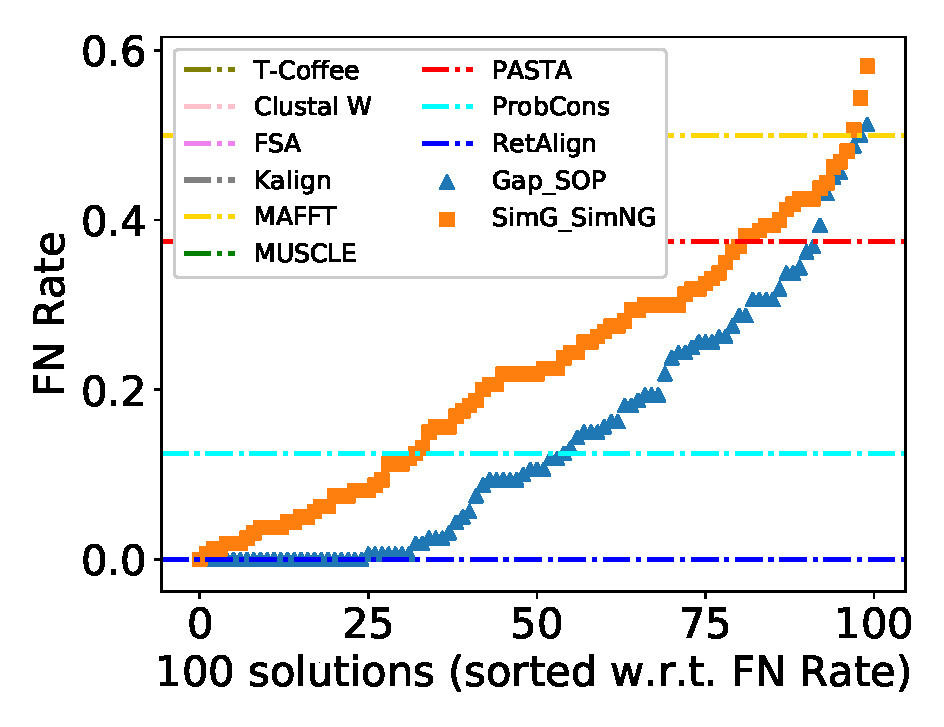
\includegraphics[width=\columnwidth]{Figure/summary/precomputedInit/Balibase/BB12001_fnrate_density_single_run}
			\caption{BB12001}
			%\label{fig:con_pr09}
		\end{subfigure}	
		\begin{subfigure}{0.22\textwidth}
			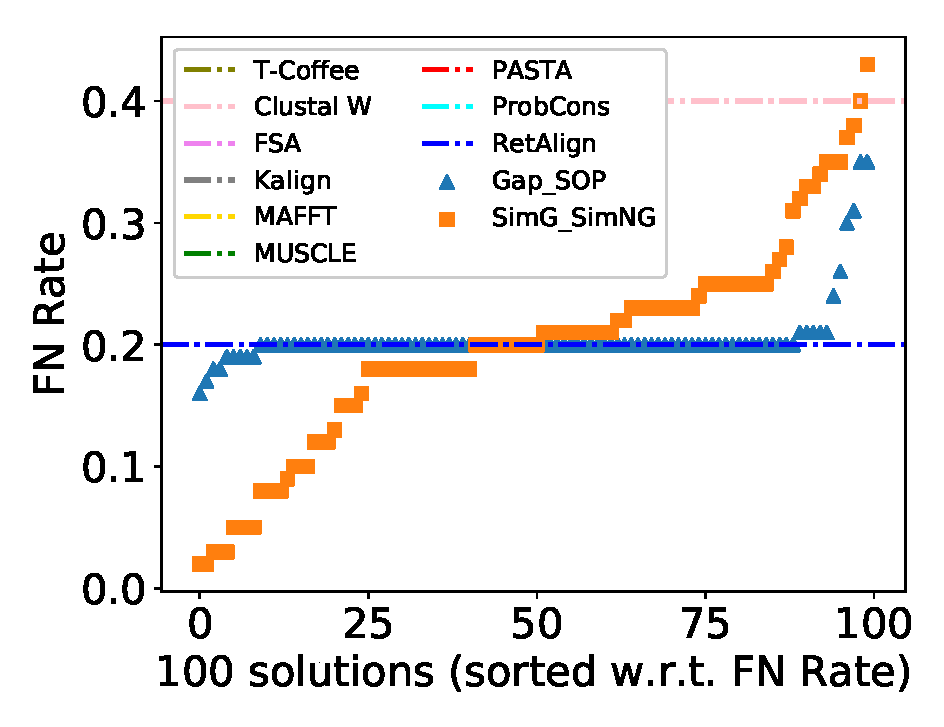
\includegraphics[width=\columnwidth]{Figure/summary/precomputedInit/Balibase/BB12013_fnrate_density_single_run}
			\caption{BB12013}
			%\label{fig:con_pr09}
		\end{subfigure}
		\begin{subfigure}{0.22\textwidth}
			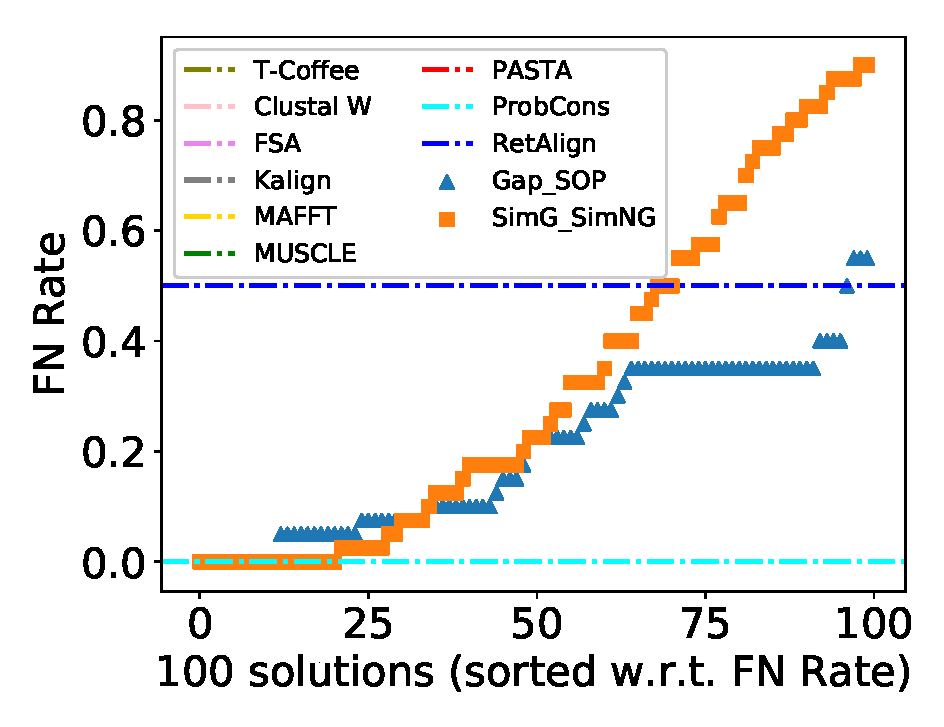
\includegraphics[width=\columnwidth]{Figure/summary/precomputedInit/Balibase/BB12022_fnrate_density_single_run}
			\caption{BB12022}
			%\label{fig:con_pr09}
		\end{subfigure}
		\begin{subfigure}{0.22\textwidth}
			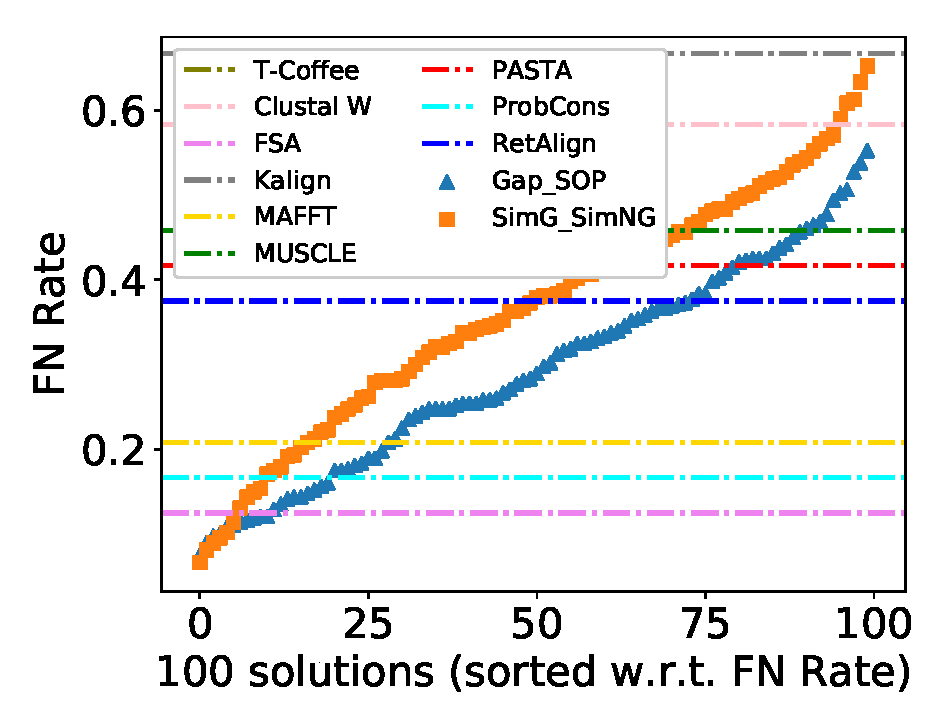
\includegraphics[width=\columnwidth]{Figure/summary/precomputedInit/Balibase/BB12035_fnrate_density_single_run}
			\caption{BB12035}
			%\label{fig:con_pr09}
		\end{subfigure}
		\begin{subfigure}{0.22\textwidth}
			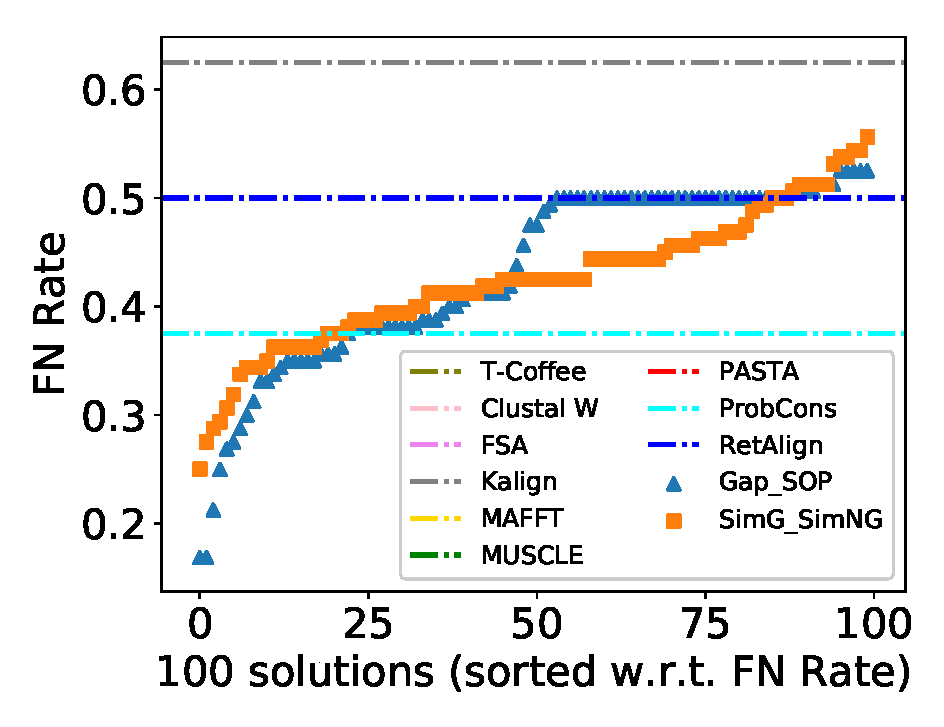
\includegraphics[width=\columnwidth]{Figure/summary/precomputedInit/Balibase/BB12044_fnrate_density_single_run}
			\caption{BB12044}
			%\label{fig:con_pr09}
		\end{subfigure}
		\begin{subfigure}{0.22\textwidth}
			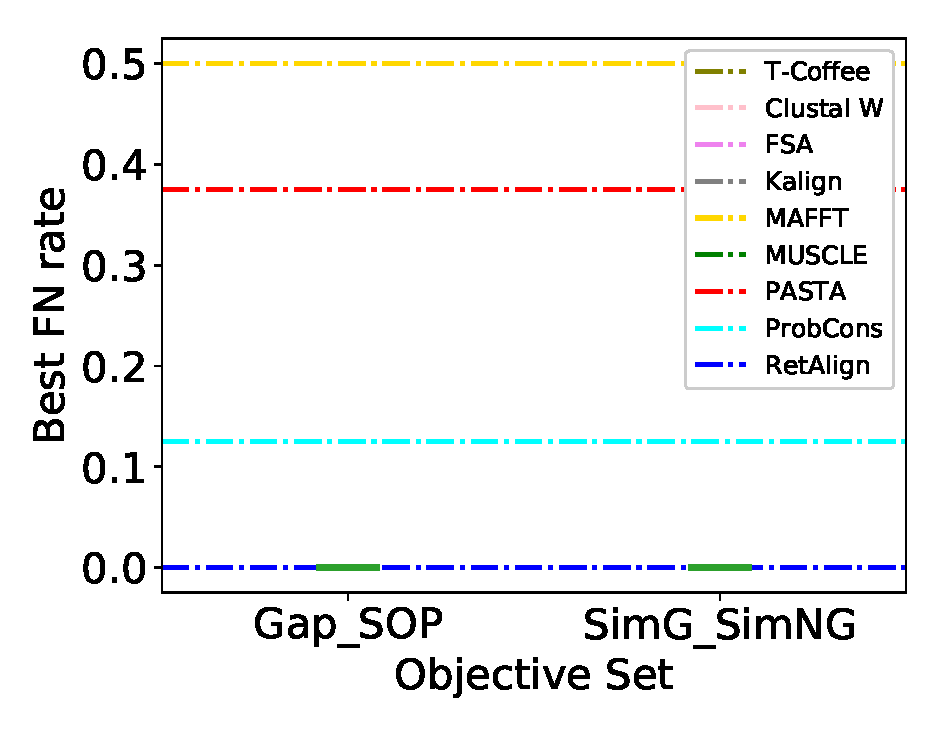
\includegraphics[width=\columnwidth]{Figure/summary/precomputedInit/Balibase/BB12001_objset_fnrate_rank}
			\caption{BB12001}
			%\label{fig:con_pr09}
		\end{subfigure}	
		\begin{subfigure}{0.22\textwidth}
			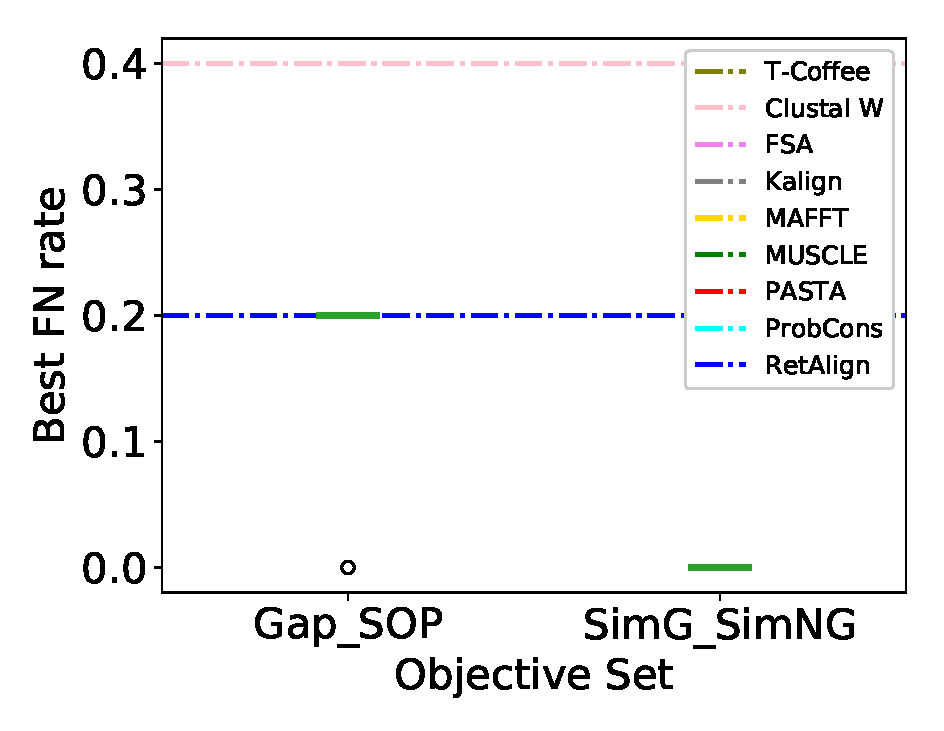
\includegraphics[width=\columnwidth]{Figure/summary/precomputedInit/Balibase/BB12013_objset_fnrate_rank}
			\caption{BB12013}
			%\label{fig:con_pr09}
		\end{subfigure}
		\begin{subfigure}{0.22\textwidth}
			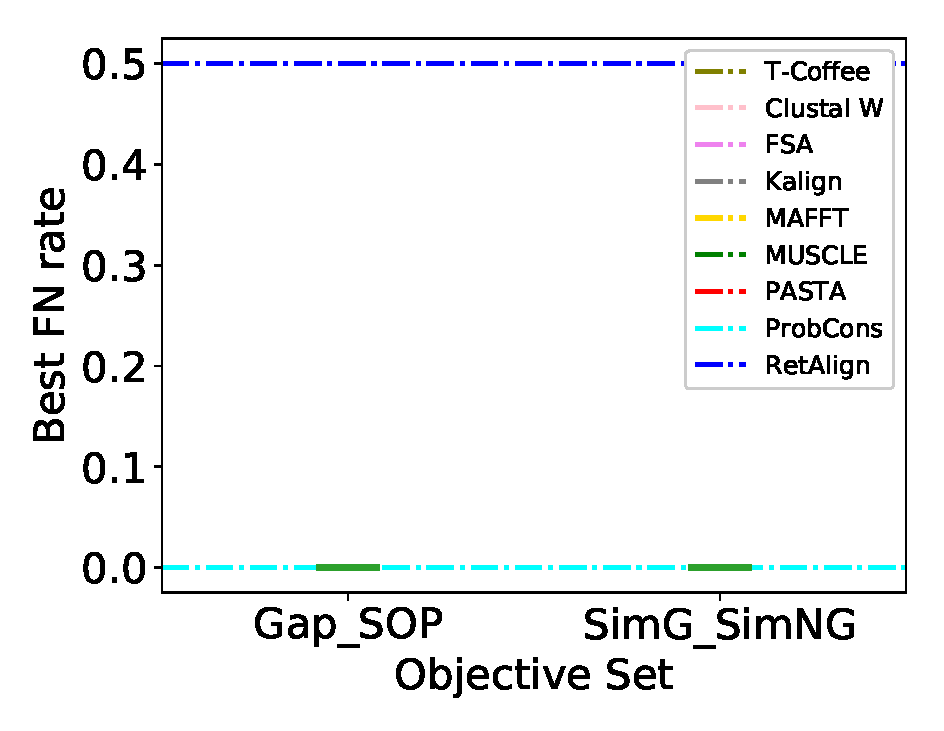
\includegraphics[width=\columnwidth]{Figure/summary/precomputedInit/Balibase/BB12022_objset_fnrate_rank}
			\caption{BB12022}
			%\label{fig:con_pr09}
		\end{subfigure}
		\begin{subfigure}{0.22\textwidth}
			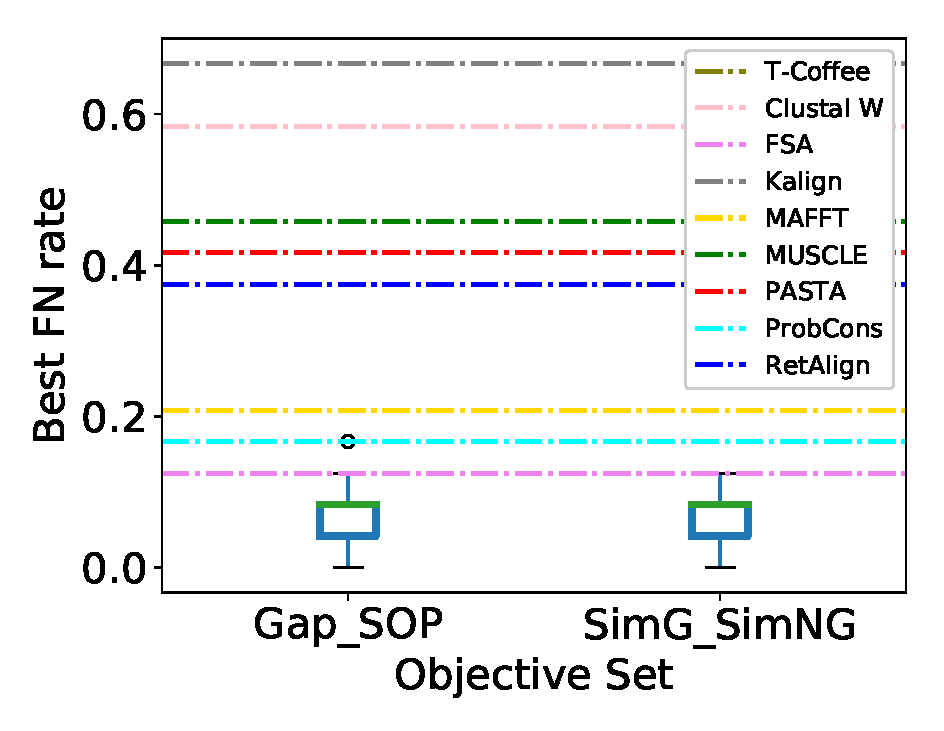
\includegraphics[width=\columnwidth]{Figure/summary/precomputedInit/Balibase/BB12035_objset_fnrate_rank}
			\caption{BB12035}
			%\label{fig:con_pr09}
		\end{subfigure}
		\begin{subfigure}{0.22\textwidth}
			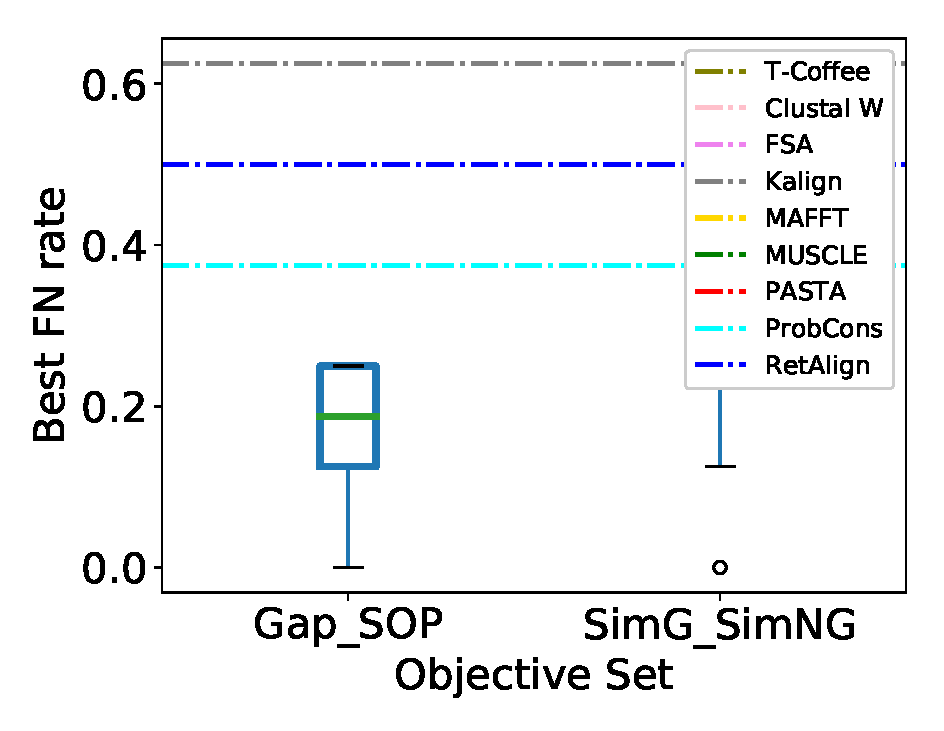
\includegraphics[width=\columnwidth]{Figure/summary/precomputedInit/Balibase/BB12044_objset_fnrate_rank}
			\caption{BB12044}
			%\label{fig:con_pr09}
		\end{subfigure}
		\end{adjustwidth}
		\caption[FN rate results on RV12]{\underline{RV12:} Top panel (part (a) - (e)) shows the FN rate of 100 solutions averaged over 20 runs. At first, we sort the FN rates of each solution set. Then we average the FN rates at each sorted position of all the sets. Bottom panel (part (f) - (j)) shows the distribution of the best FN rates collected from all runs. In each figure, the horizontal lines show the performance of the state-of-the-art tools.}
		\label{fig:rv12_fn_rate}

\end{figure*}


\begin{figure*}[!htbp]
	\centering
	\begin{adjustwidth}{-1.5cm}{-1cm}
		\begin{subfigure}{0.22\textwidth}
			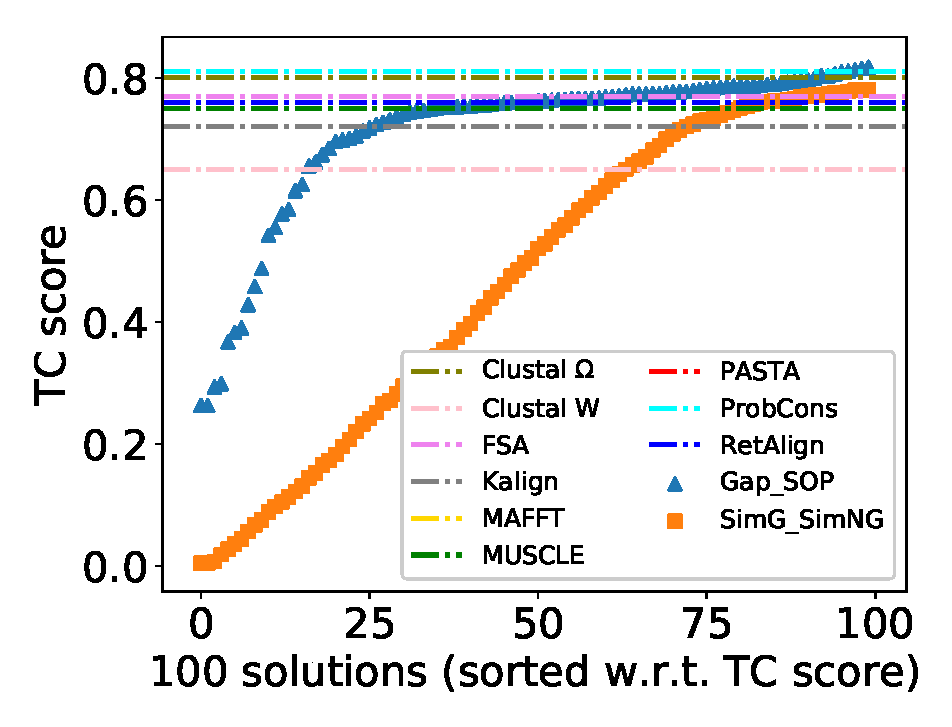
\includegraphics[width=\columnwidth]{Figure/summary/precomputedInit/Balibase/BB12001_tc_density_single_run_2}
			\caption{BB12001}
			%\label{fig:con_pr09}
		\end{subfigure}	
		\begin{subfigure}{0.22\textwidth}
			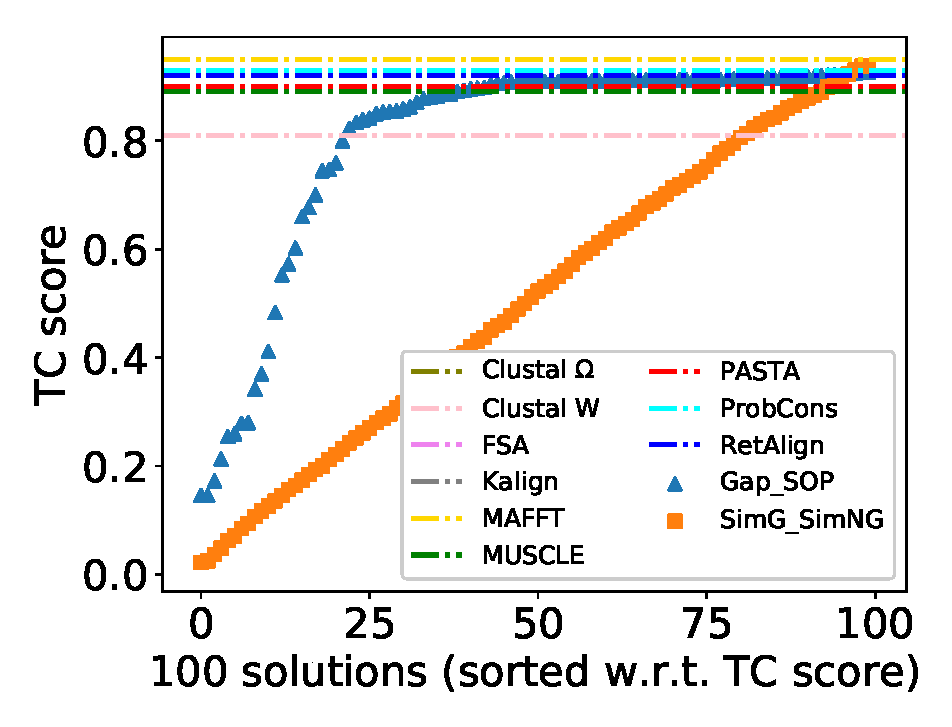
\includegraphics[width=\columnwidth]{Figure/summary/precomputedInit/Balibase/BB12013_tc_density_single_run_2}
			\caption{BB12013}
			%\label{fig:con_pr09}
		\end{subfigure}
		\begin{subfigure}{0.22\textwidth}
			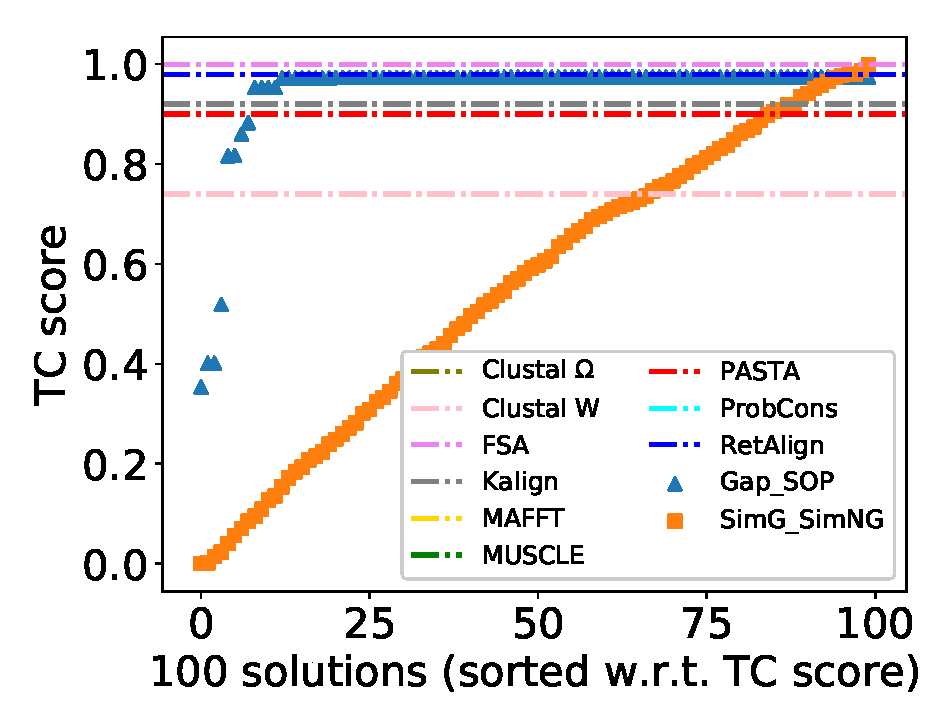
\includegraphics[width=\columnwidth]{Figure/summary/precomputedInit/Balibase/BB12022_tc_density_single_run_2}
			\caption{BB12022}
			%\label{fig:con_pr09}
		\end{subfigure}
		\begin{subfigure}{0.22\textwidth}
			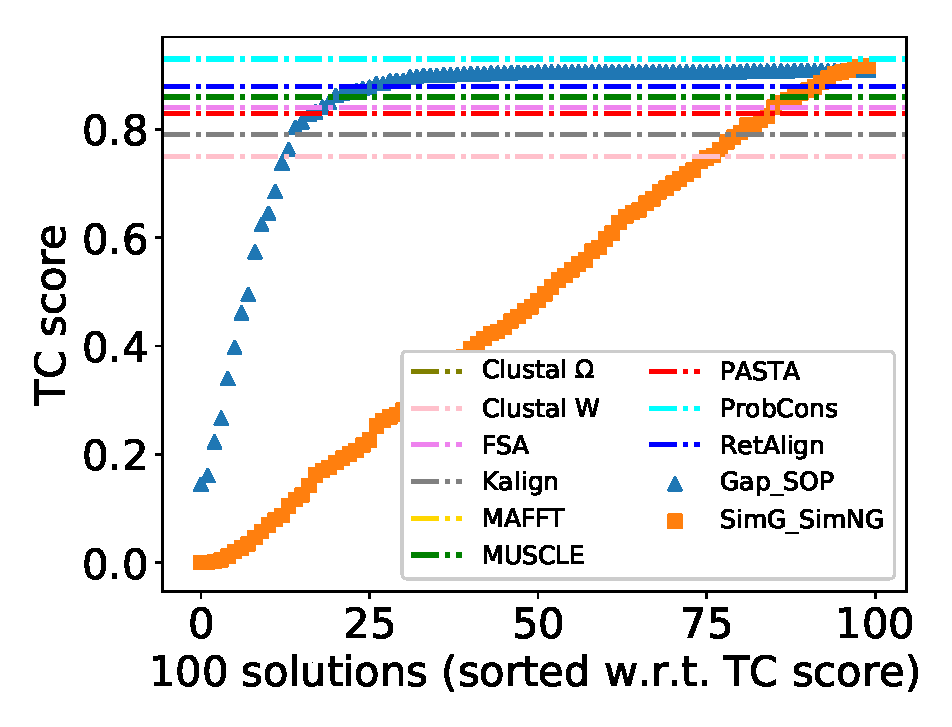
\includegraphics[width=\columnwidth]{Figure/summary/precomputedInit/Balibase/BB12035_tc_density_single_run_2}
			\caption{BB12035}
			%\label{fig:con_pr09}
		\end{subfigure}
		\begin{subfigure}{0.22\textwidth}
			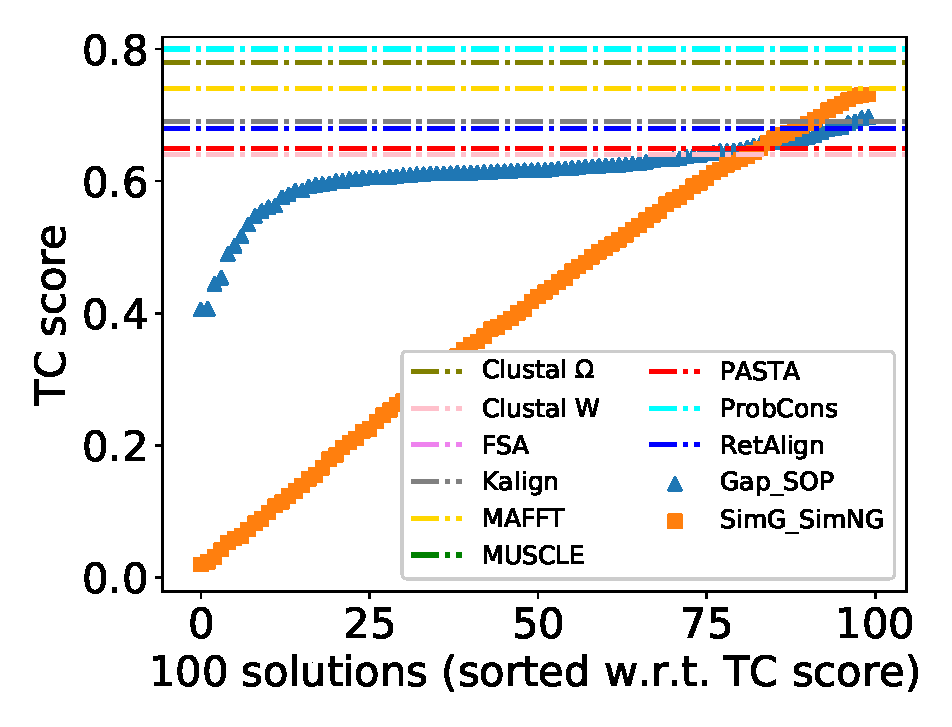
\includegraphics[width=\columnwidth]{Figure/summary/precomputedInit/Balibase/BB12044_tc_density_single_run_2}
			\caption{BB12044}
			%\label{fig:con_pr09}
		\end{subfigure}
		%%%%%%%%%%%%%%
		\begin{subfigure}{0.22\textwidth}
			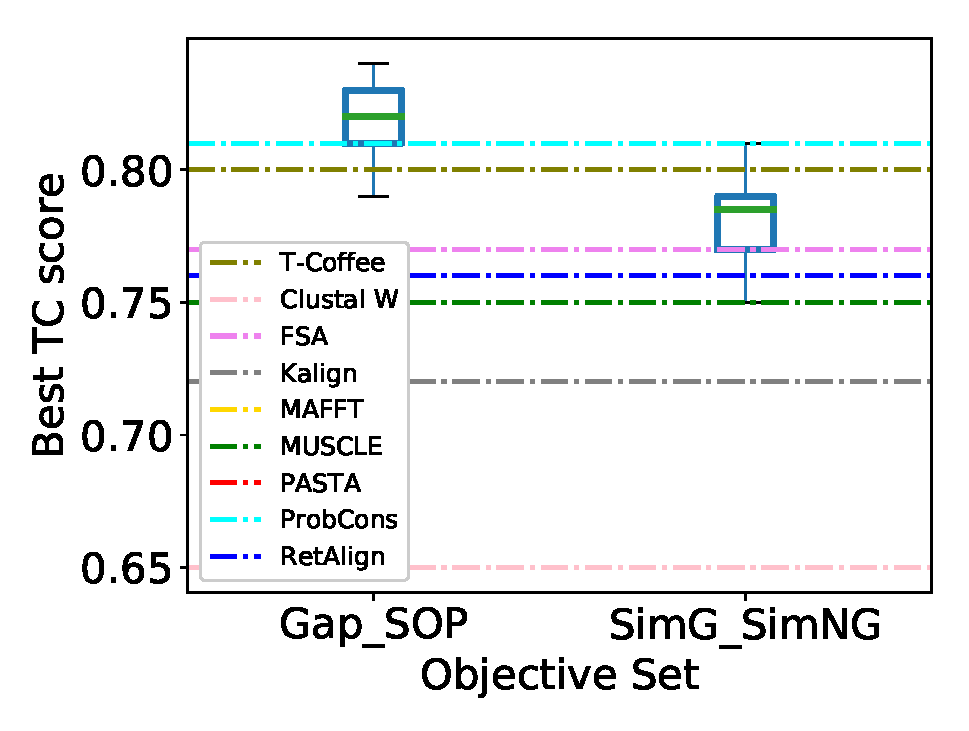
\includegraphics[width=\columnwidth]{Figure/summary/precomputedInit/Balibase/BB12001_objset_tc_rank_2}
			\caption{BB12001}
			%\label{fig:con_pr09}
		\end{subfigure}	
		\begin{subfigure}{0.22\textwidth}
			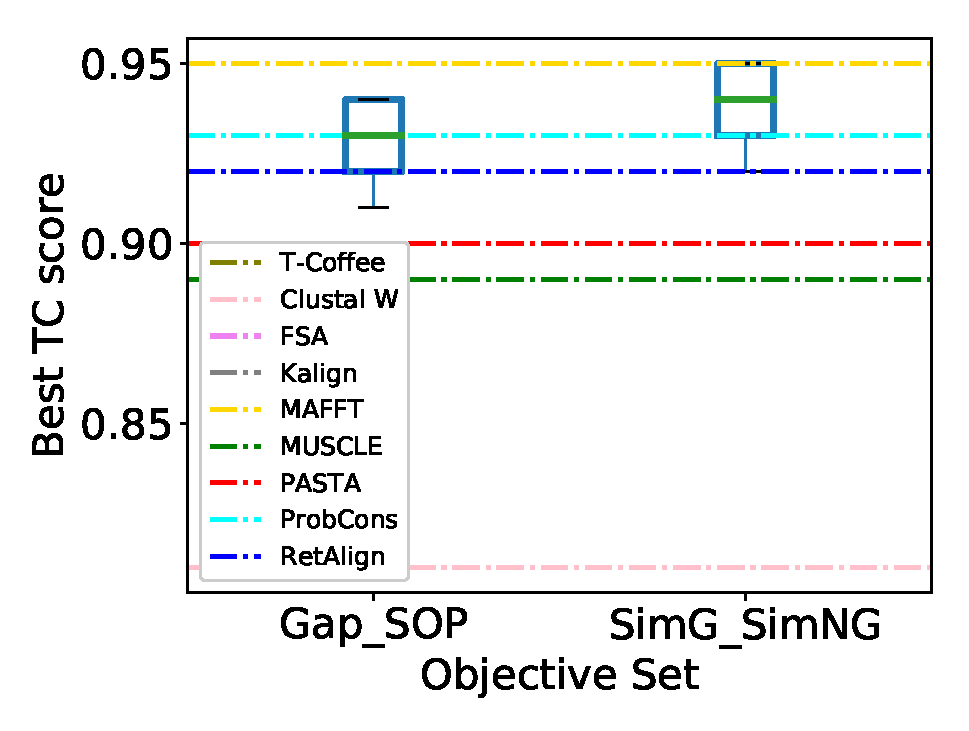
\includegraphics[width=\columnwidth]{Figure/summary/precomputedInit/Balibase/BB12013_objset_tc_rank_2}
			\caption{BB12013}
			%\label{fig:con_pr09}
		\end{subfigure}
		\begin{subfigure}{0.22\textwidth}
			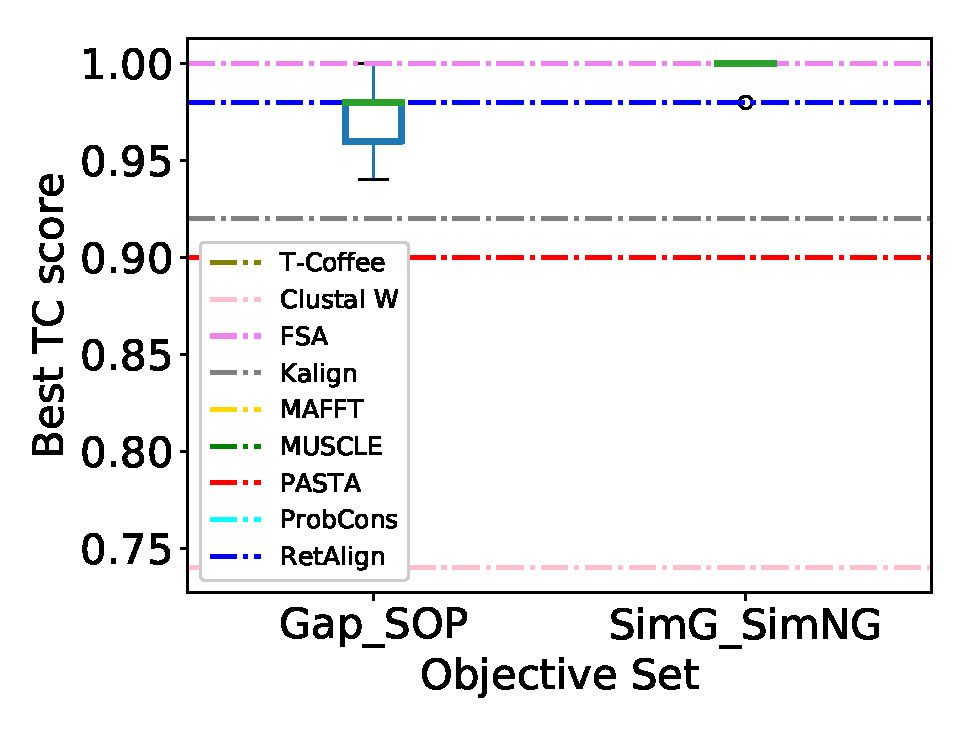
\includegraphics[width=\columnwidth]{Figure/summary/precomputedInit/Balibase/BB12022_objset_tc_rank_2}
			\caption{BB12022}
			%\label{fig:con_pr09}
		\end{subfigure}
		\begin{subfigure}{0.22\textwidth}
			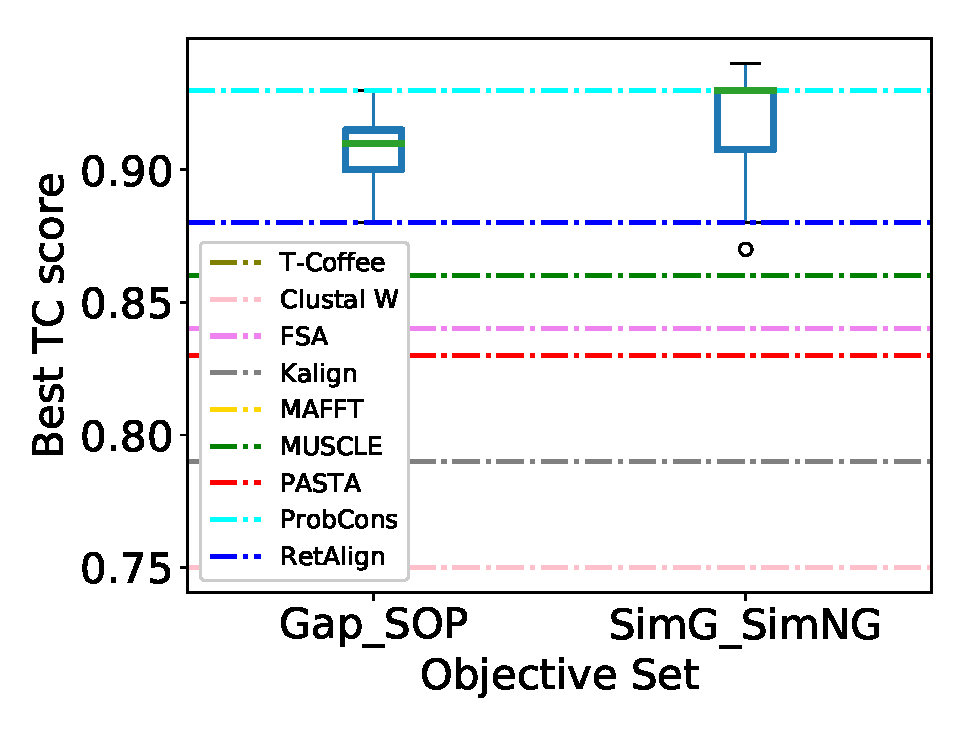
\includegraphics[width=\columnwidth]{Figure/summary/precomputedInit/Balibase/BB12035_objset_tc_rank_2}
			\caption{BB12035}
			%\label{fig:con_pr09}
		\end{subfigure}
		\begin{subfigure}{0.22\textwidth}
			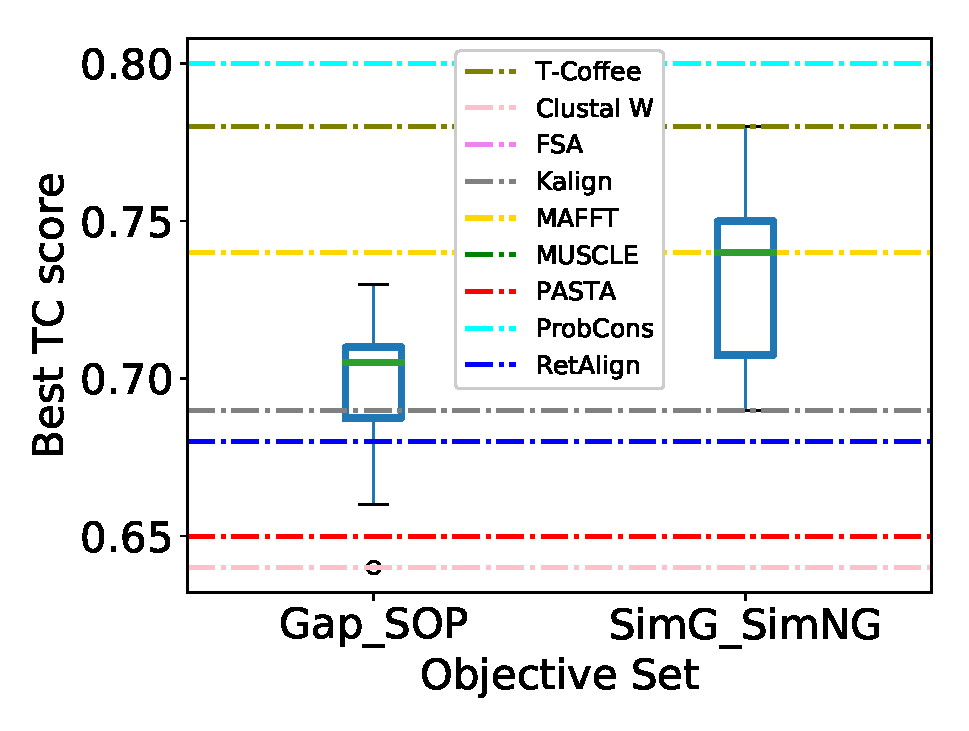
\includegraphics[width=\columnwidth]{Figure/summary/precomputedInit/Balibase/BB12044_objset_tc_rank_2}
			\caption{BB12044}
			%\label{fig:con_pr09}
		\end{subfigure}
		\end{adjustwidth}
		\caption[TC score results on RV12]{\underline{RV12:} Top panel (part (a) - (e)) shows the TC score of 100 solutions averaged over 20 runs. At first, we sort the TC scores of each solution set. Then we average the TC scores at each sorted position of all the sets. Bottom panel (part (f) - (j)) shows the distribution of the best TC scores collected from all runs. In each figure, the horizontal lines show the performance of the state-of-the-art tools.}
		\label{fig:rv12_tc}

\end{figure*}


\begin{figure*}[!htbp]
	\centering
	\begin{adjustwidth}{-1.5cm}{-1cm}
		\begin{subfigure}{0.22\textwidth}
			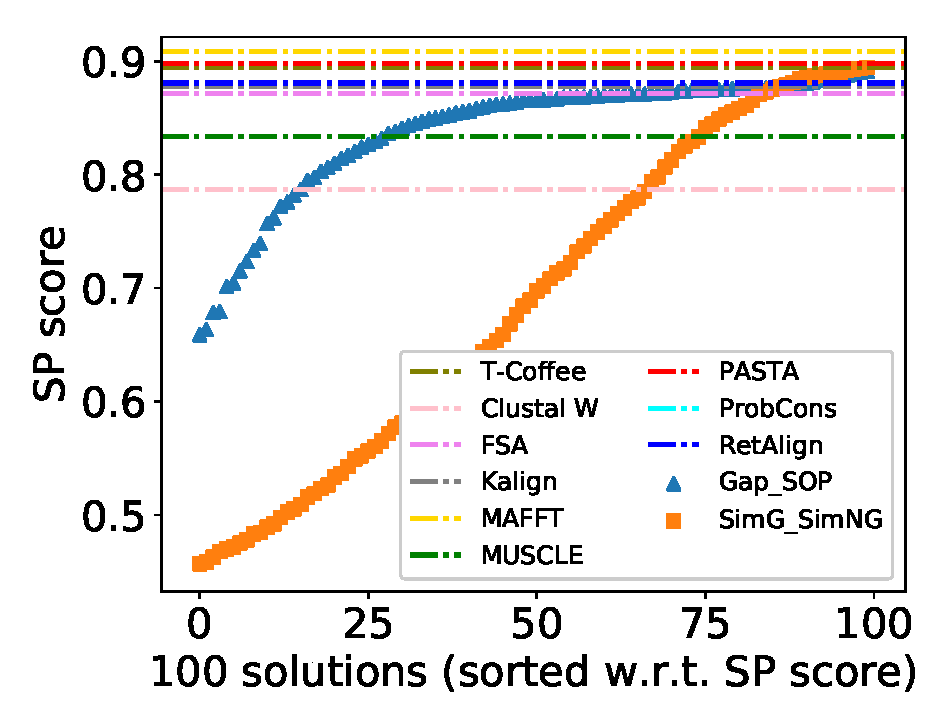
\includegraphics[width=\columnwidth]{Figure/summary/precomputedInit/Balibase/BB12001_pairs_density_single_run_2}
			\caption{BB12001}
			%\label{fig:con_pr09}
		\end{subfigure}	
		\begin{subfigure}{0.22\textwidth}
			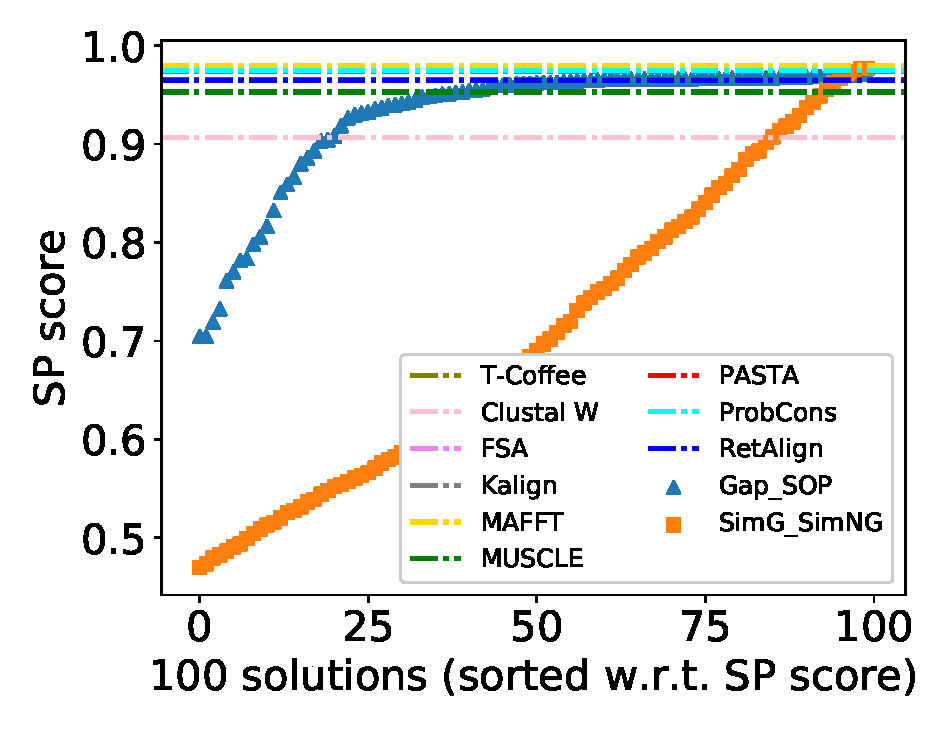
\includegraphics[width=\columnwidth]{Figure/summary/precomputedInit/Balibase/BB12013_pairs_density_single_run_2}
			\caption{BB12013}
			%\label{fig:con_pr09}
		\end{subfigure}
		\begin{subfigure}{0.22\textwidth}
			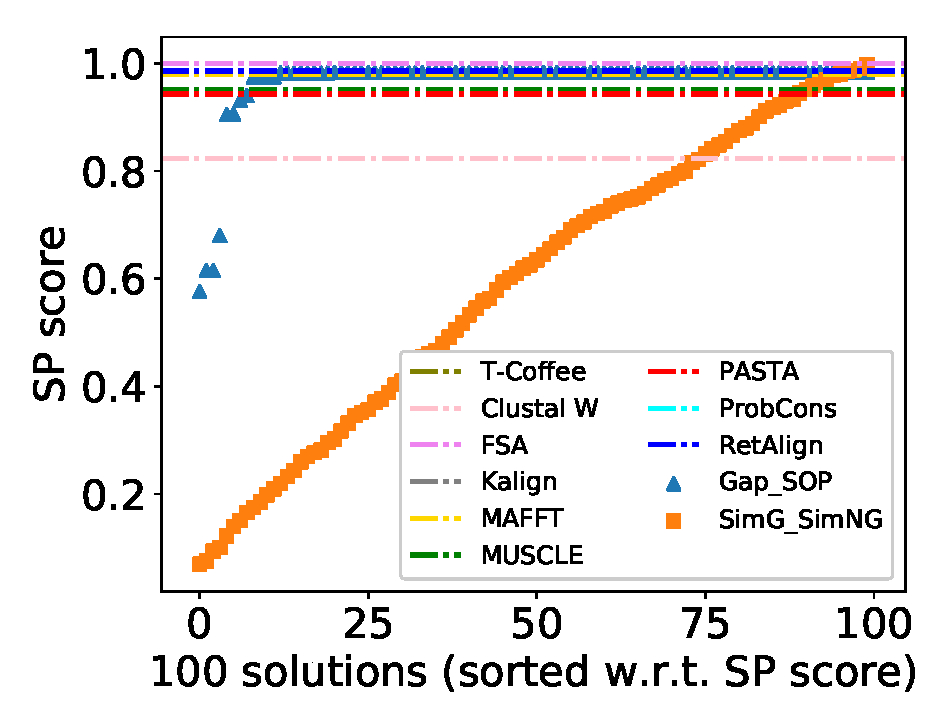
\includegraphics[width=\columnwidth]{Figure/summary/precomputedInit/Balibase/BB12022_pairs_density_single_run_2}
			\caption{BB12022}
			%\label{fig:con_pr09}
		\end{subfigure}
		\begin{subfigure}{0.22\textwidth}
			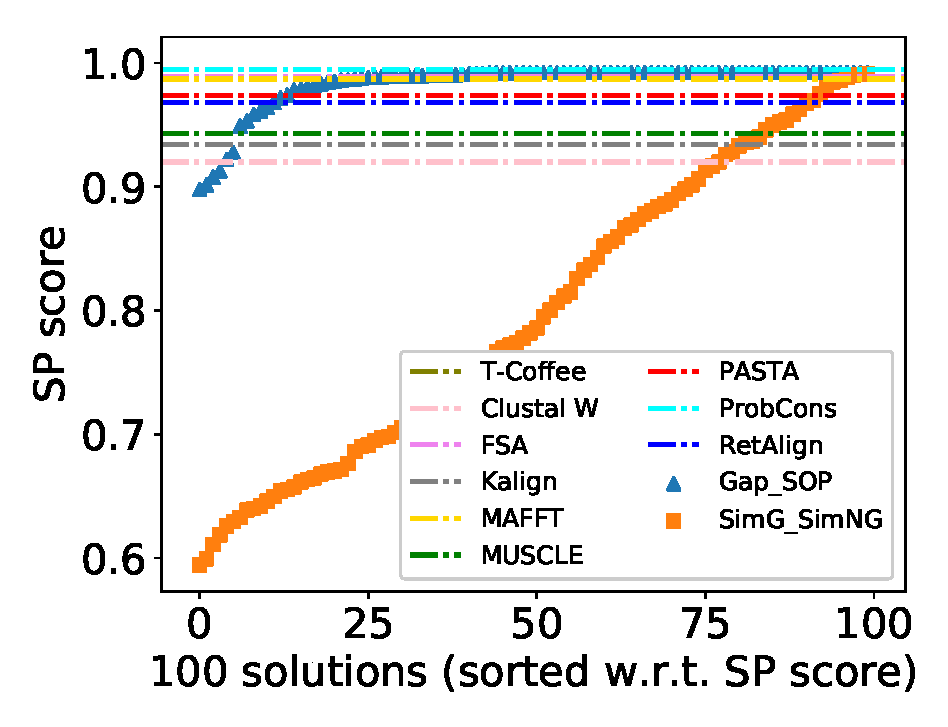
\includegraphics[width=\columnwidth]{Figure/summary/precomputedInit/Balibase/BB12035_pairs_density_single_run_2}
			\caption{BB12035}
			%\label{fig:con_pr09}
		\end{subfigure}
		\begin{subfigure}{0.22\textwidth}
			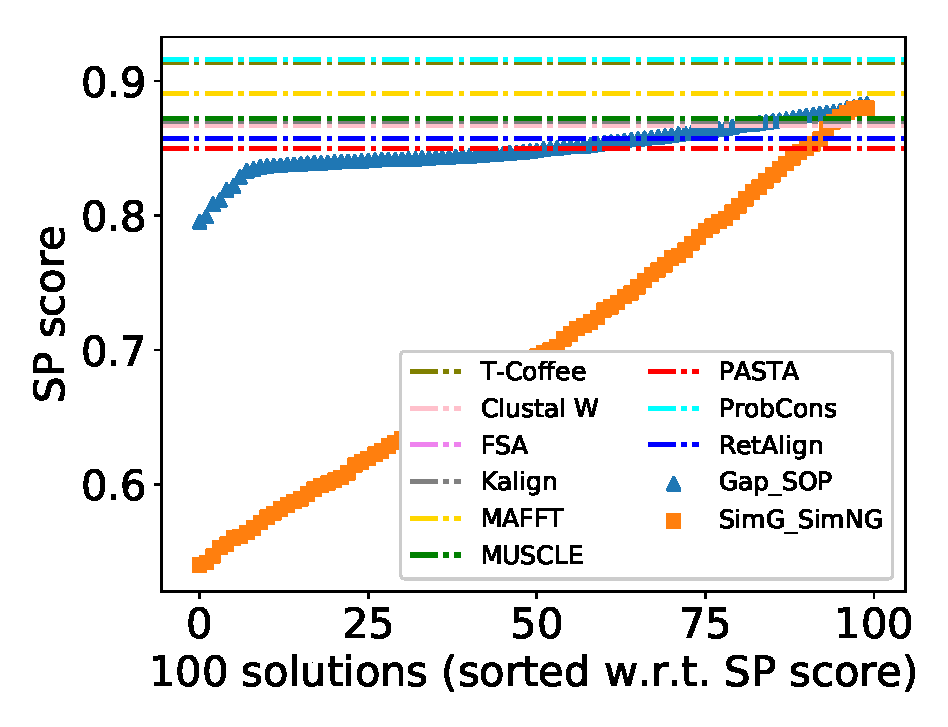
\includegraphics[width=\columnwidth]{Figure/summary/precomputedInit/Balibase/BB12044_pairs_density_single_run_2}
			\caption{BB12044}
			%\label{fig:con_pr09}
		\end{subfigure}
		\begin{subfigure}{0.22\textwidth}
			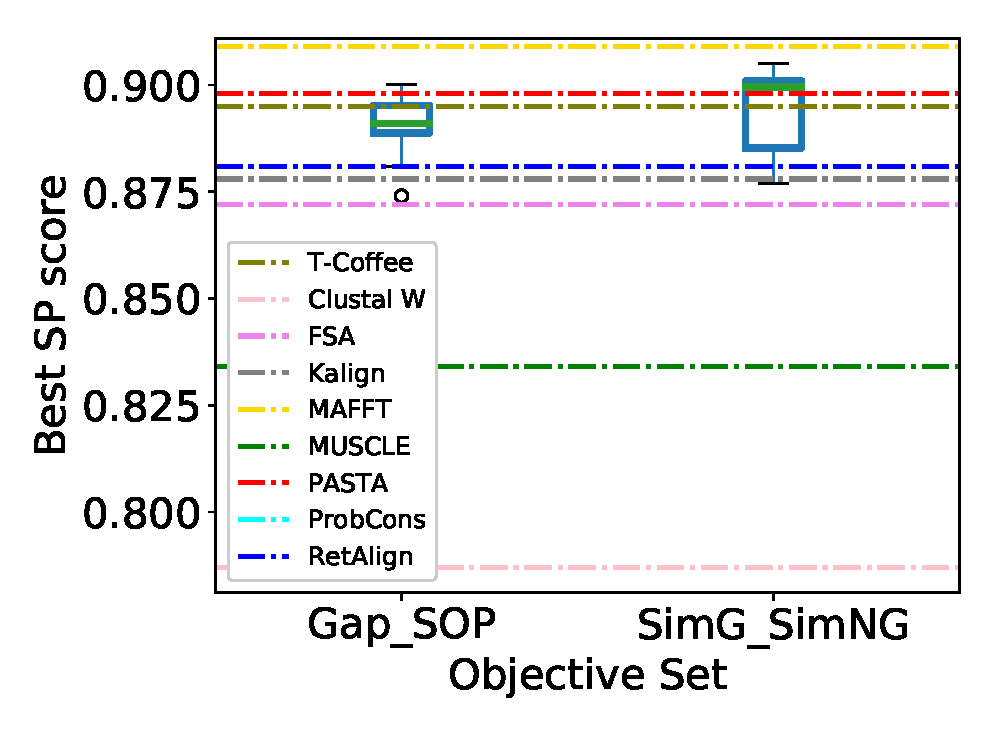
\includegraphics[width=\columnwidth]{Figure/summary/precomputedInit/Balibase/BB12001_objset_pairs_rank_2}
			\caption{BB12001}
			%\label{fig:con_pr09}
		\end{subfigure}	
		\begin{subfigure}{0.22\textwidth}
			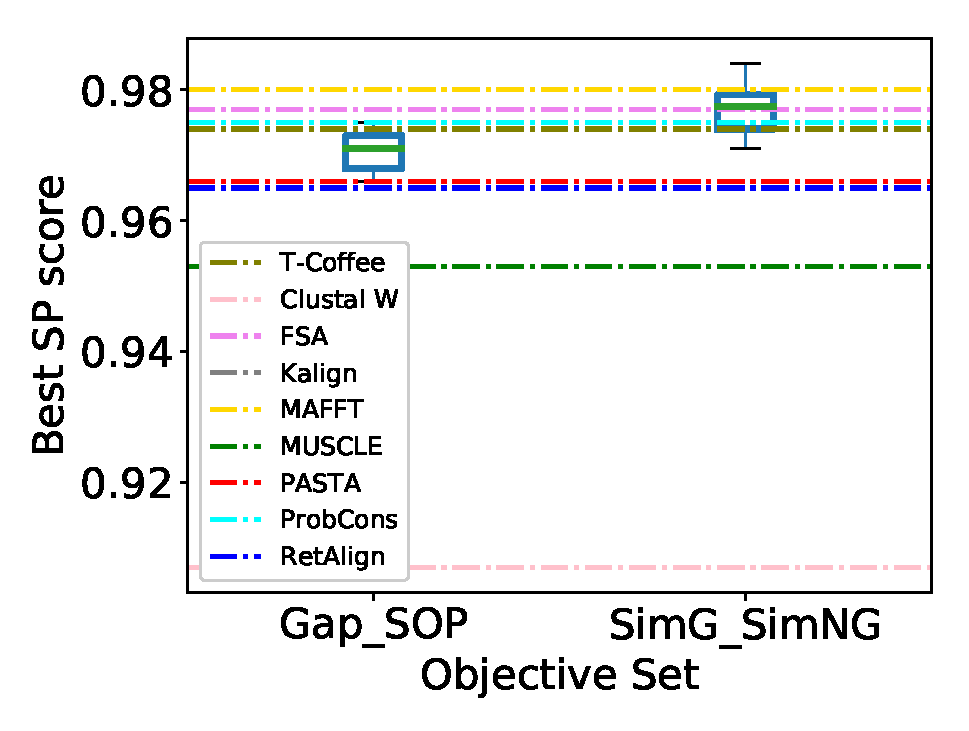
\includegraphics[width=\columnwidth]{Figure/summary/precomputedInit/Balibase/BB12013_objset_pairs_rank_2}
			\caption{BB12013}
			%\label{fig:con_pr09}
		\end{subfigure}
		\begin{subfigure}{0.22\textwidth}
			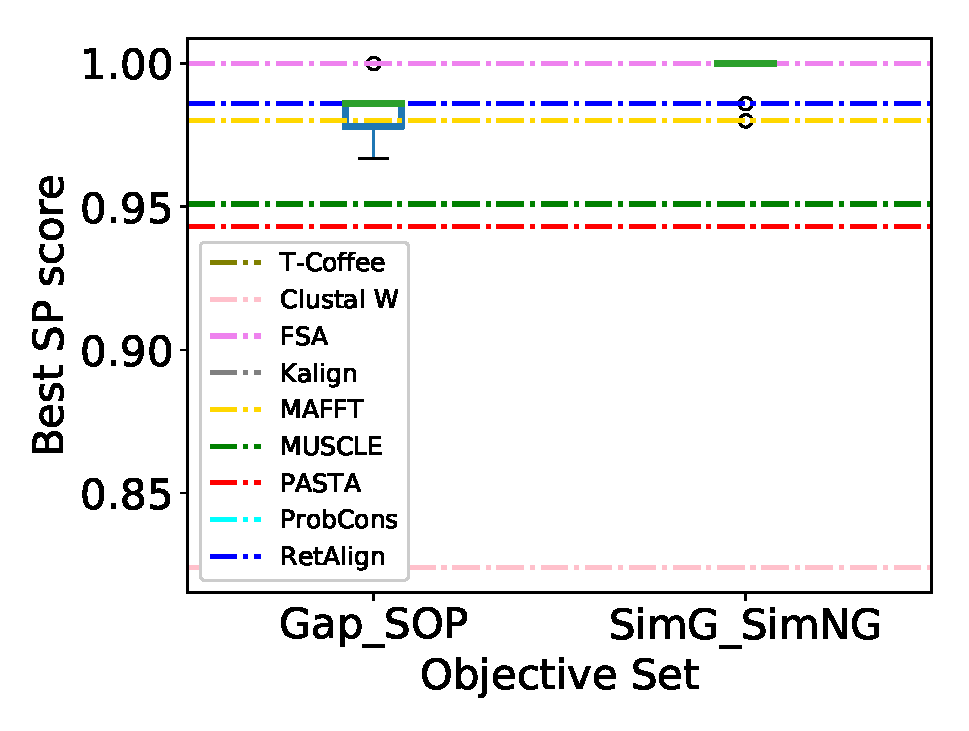
\includegraphics[width=\columnwidth]{Figure/summary/precomputedInit/Balibase/BB12022_objset_pairs_rank_2}
			\caption{BB12022}
			%\label{fig:con_pr09}
		\end{subfigure}
		\begin{subfigure}{0.22\textwidth}
			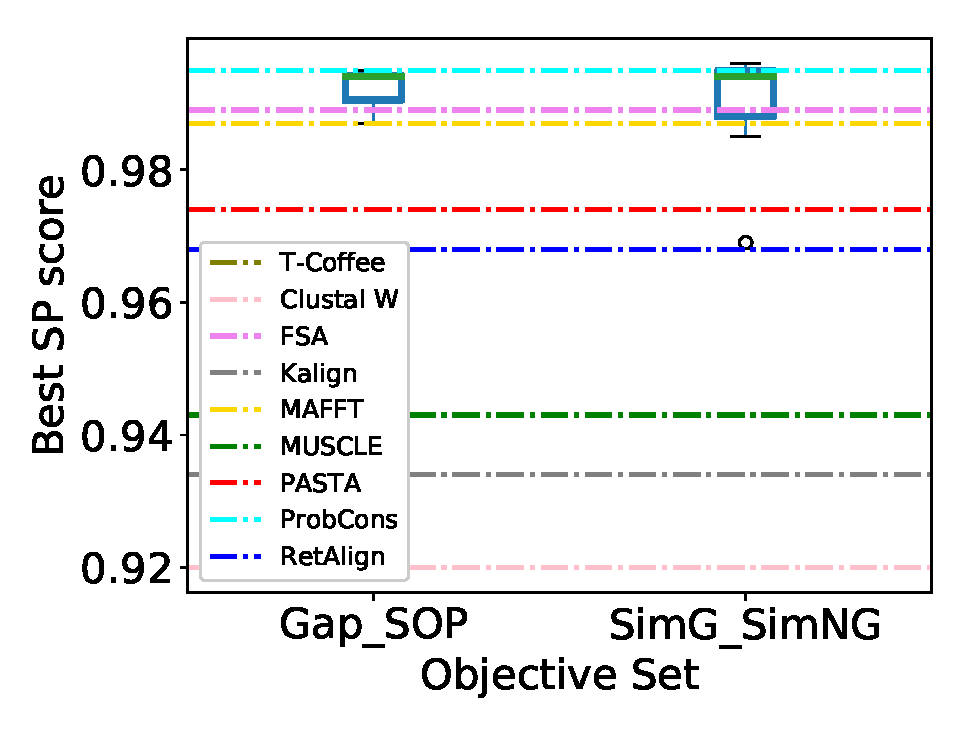
\includegraphics[width=\columnwidth]{Figure/summary/precomputedInit/Balibase/BB12035_objset_pairs_rank_2}
			\caption{BB12035}
			%\label{fig:con_pr09}
		\end{subfigure}
		\begin{subfigure}{0.22\textwidth}
			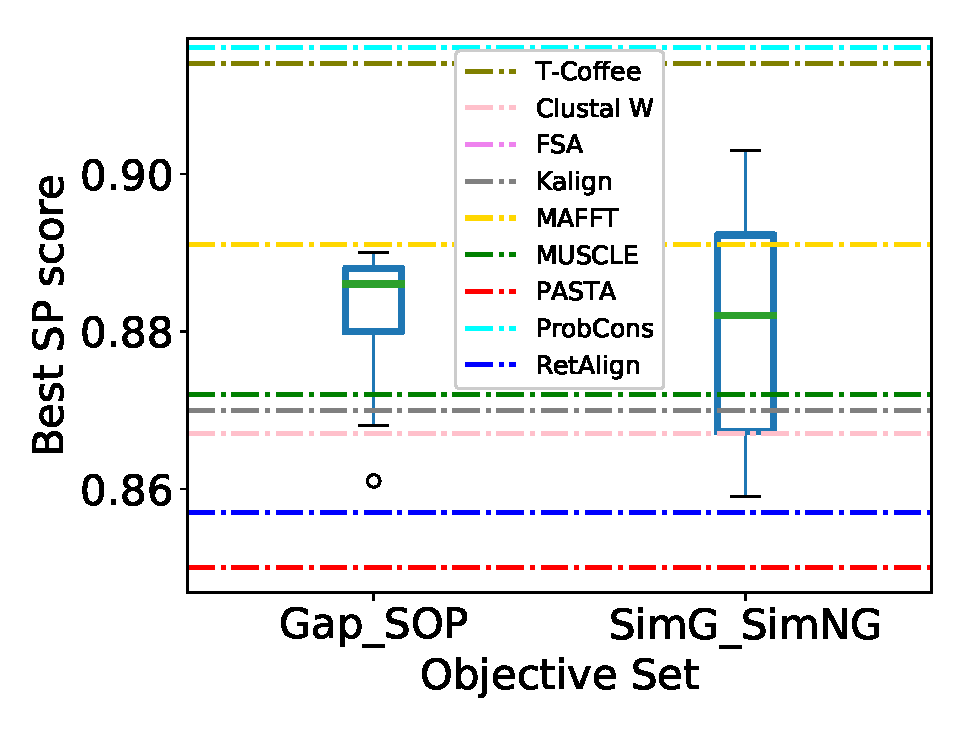
\includegraphics[width=\columnwidth]{Figure/summary/precomputedInit/Balibase/BB12044_objset_pairs_rank_2}
			\caption{BB12044}
			%\label{fig:con_pr09}
		\end{subfigure}
	\end{adjustwidth}
		\caption[SP score results on RV12]{\underline{RV12:} Top panel (part (a) - (e)) shows the SP score of 100 solutions averaged over 20 runs. At first, we sort the SP scores of each solution set. Then we average the SP scores at each sorted position of all the sets. Bottom panel (part (f) - (j)) shows the distribution of the best SP scores collected from all runs. In each figure, the horizontal lines show the performance of the state-of-the-art tools.}
		\label{fig:rv12_sp}
	
\end{figure*}


\begin{figure*}[!htbp]
	\centering
	\begin{adjustwidth}{-1.5cm}{-1cm}
		\begin{subfigure}{0.22\textwidth}
			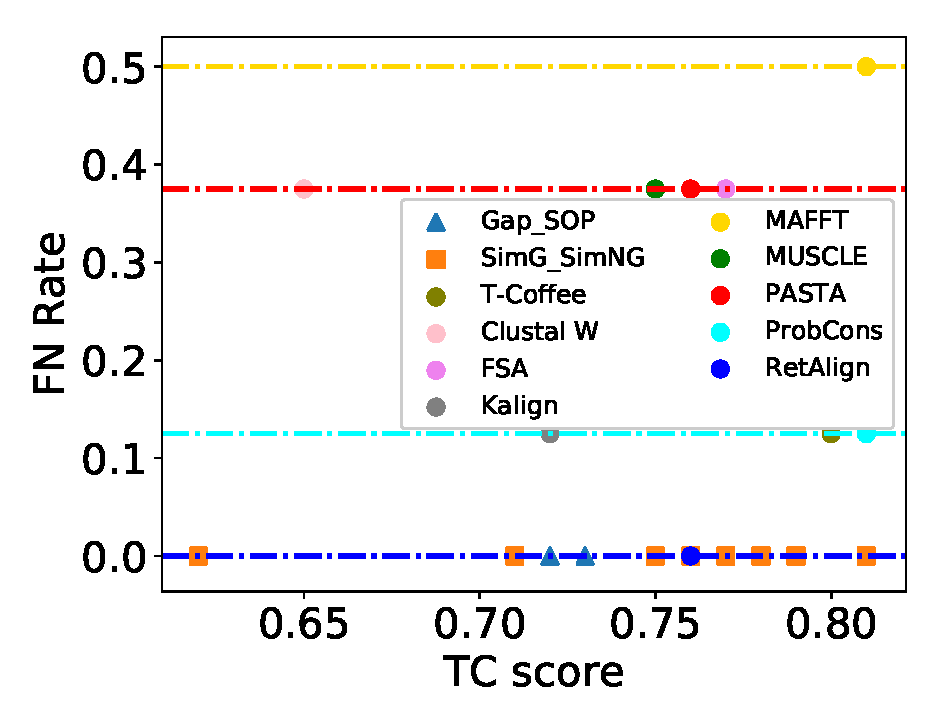
\includegraphics[width=\columnwidth]{Figure/summary/precomputedInit/Balibase/BB12001_fnrate_vs_tc_2}
			\caption{BB12001}
			%\label{fig:con_pr09}
		\end{subfigure}	
		\begin{subfigure}{0.22\textwidth}
			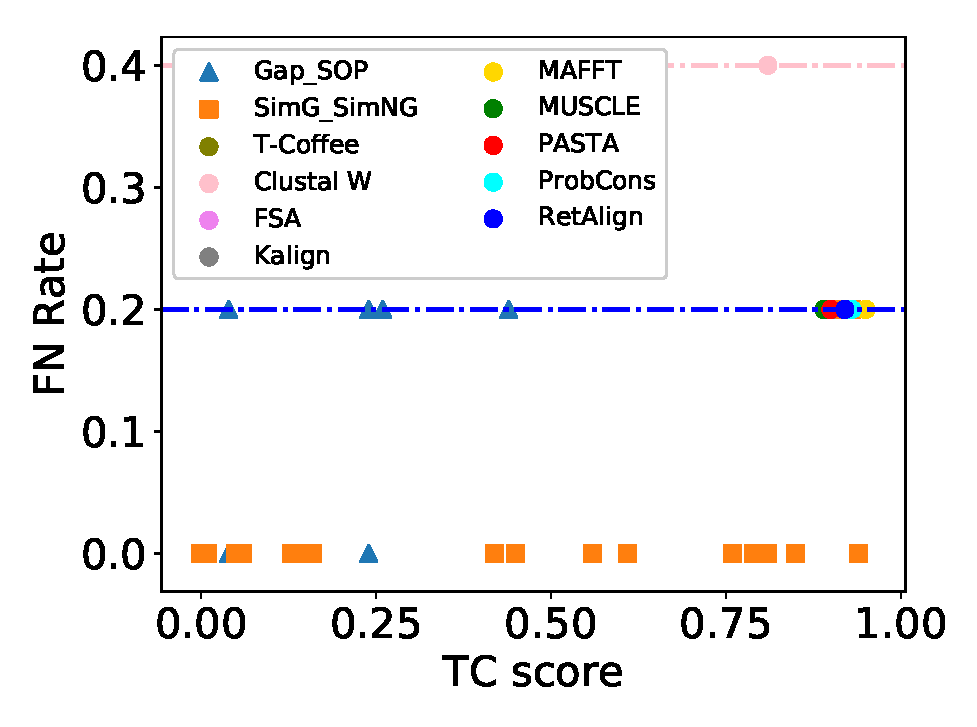
\includegraphics[width=\columnwidth]{Figure/summary/precomputedInit/Balibase/BB12013_fnrate_vs_tc_2}
			\caption{BB12013}
			%\label{fig:con_pr09}
		\end{subfigure}
		\begin{subfigure}{0.22\textwidth}
			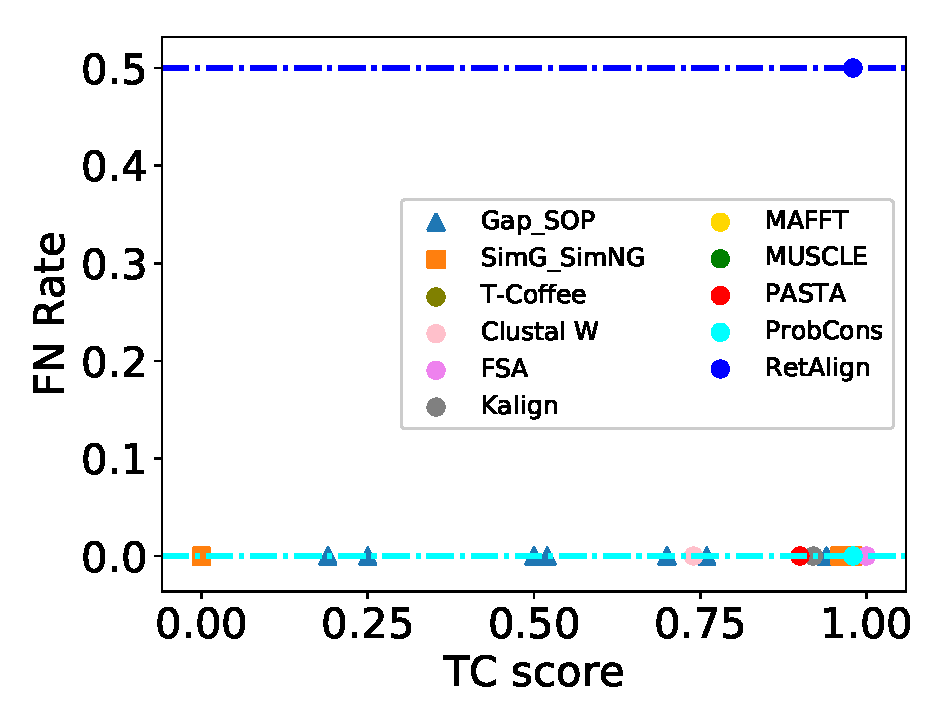
\includegraphics[width=\columnwidth]{Figure/summary/precomputedInit/Balibase/BB12022_fnrate_vs_tc_2}
			\caption{BB12022}
			%\label{fig:con_pr09}
		\end{subfigure}
		\begin{subfigure}{0.22\textwidth}
			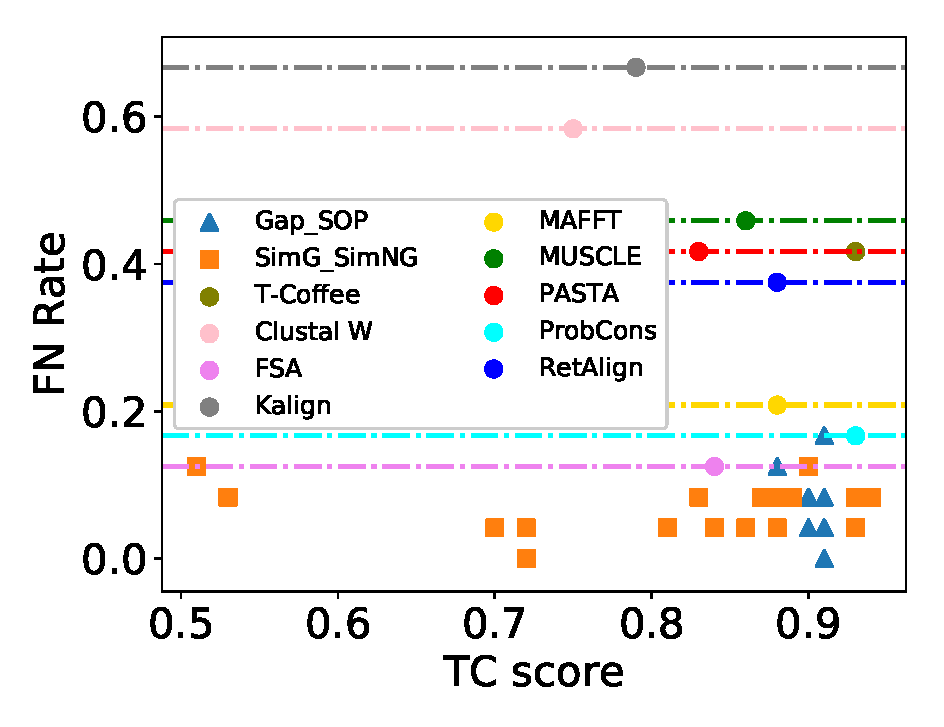
\includegraphics[width=\columnwidth]{Figure/summary/precomputedInit/Balibase/BB12035_fnrate_vs_tc_2}
			\caption{BB12035}
			%\label{fig:con_pr09}
		\end{subfigure}	
		\begin{subfigure}{0.22\textwidth}
			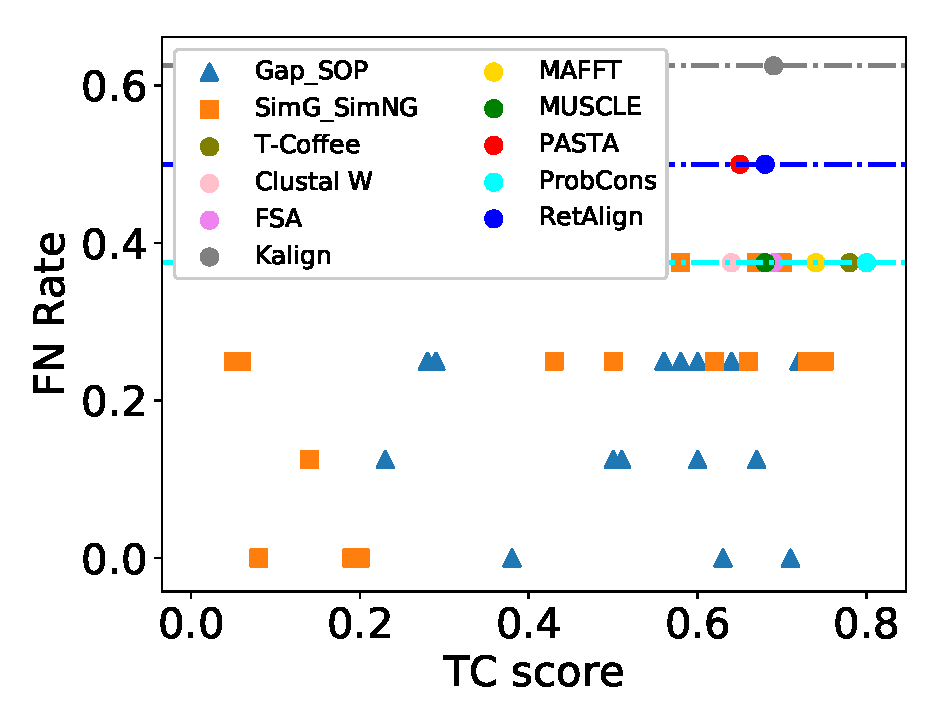
\includegraphics[width=\columnwidth]{Figure/summary/precomputedInit/Balibase/BB12044_fnrate_vs_tc_2}
			\caption{BB12044}
			%\label{fig:con_pr09}
		\end{subfigure}
		%%%%%%%%%
		\begin{subfigure}{0.22\textwidth}
			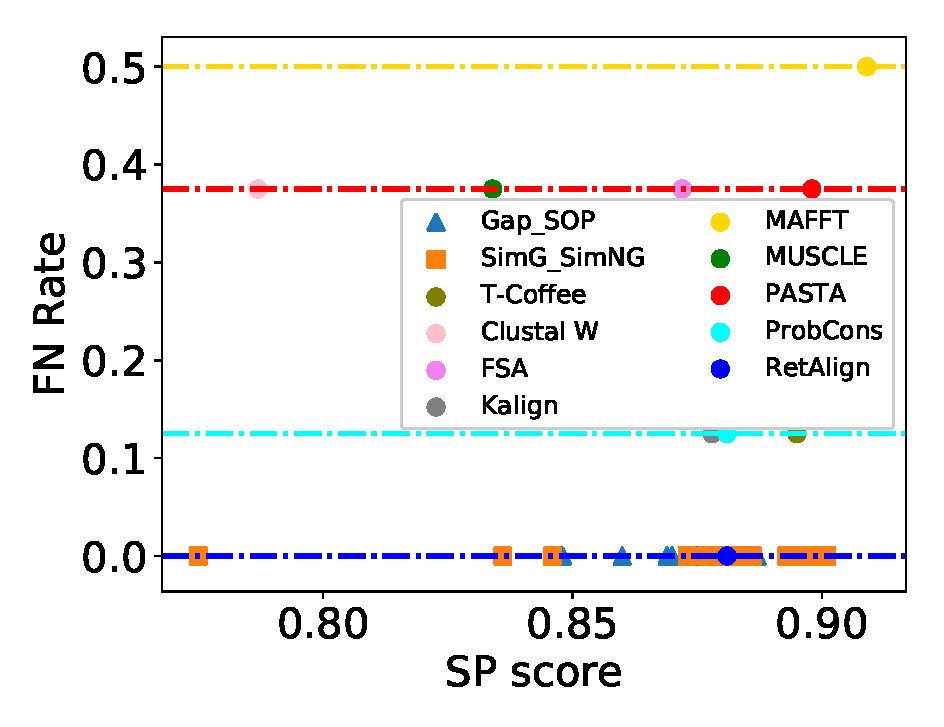
\includegraphics[width=\columnwidth]{Figure/summary/precomputedInit/Balibase/BB12001_fnrate_vs_sp_2}
			\caption{BB12001}
			%\label{fig:con_pr09}
		\end{subfigure}	
		\begin{subfigure}{0.22\textwidth}
			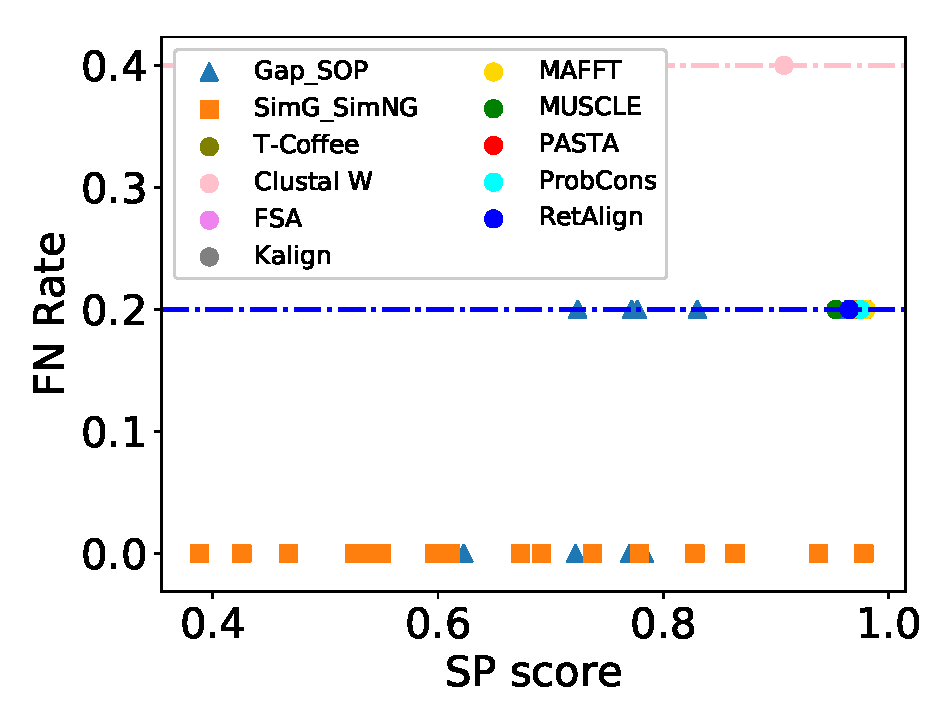
\includegraphics[width=\columnwidth]{Figure/summary/precomputedInit/Balibase/BB12013_fnrate_vs_sp_2}
			\caption{BB12013}
			%\label{fig:con_pr09}
		\end{subfigure}
		\begin{subfigure}{0.22\textwidth}
			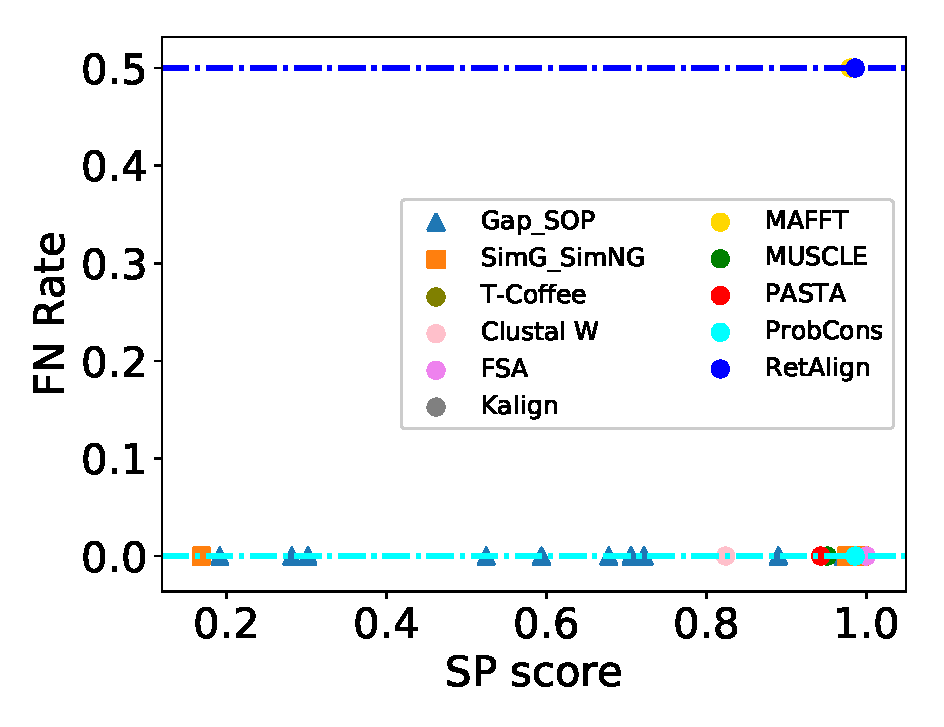
\includegraphics[width=\columnwidth]{Figure/summary/precomputedInit/Balibase/BB12022_fnrate_vs_sp_2}
			\caption{BB12022}
			%\label{fig:con_pr09}
		\end{subfigure}
		\begin{subfigure}{0.22\textwidth}
			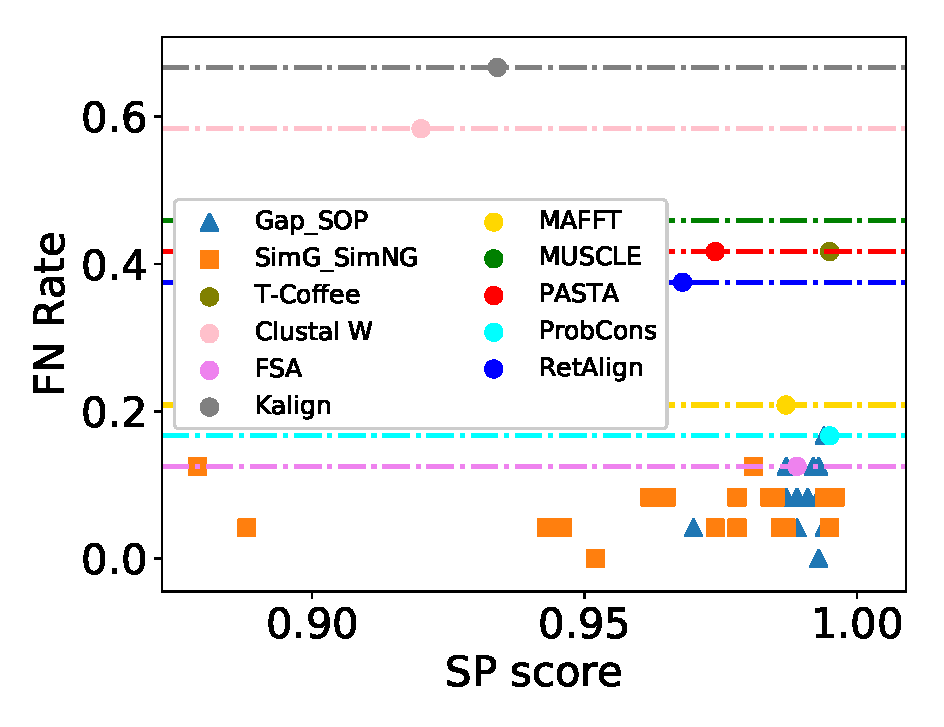
\includegraphics[width=\columnwidth]{Figure/summary/precomputedInit/Balibase/BB12035_fnrate_vs_sp_2}
			\caption{BB12035}
			%\label{fig:con_pr09}
		\end{subfigure}	
		\begin{subfigure}{0.22\textwidth}
			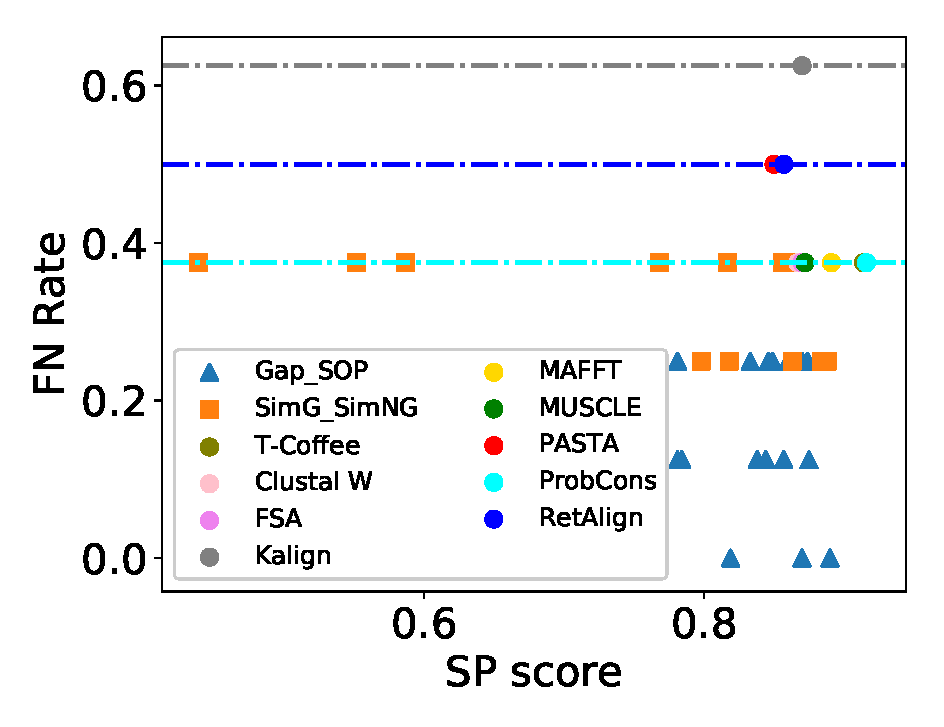
\includegraphics[width=\columnwidth]{Figure/summary/precomputedInit/Balibase/BB12044_fnrate_vs_sp_2}
			\caption{BB12044}
			%\label{fig:con_pr09}
		\end{subfigure}
		\end{adjustwidth}
		\caption[FN rate vs TC score on RV12]{\underline{RV12}: Top panel (part (a) - (e)) shows the relationship between FN rate and TC score for different alignments. And bottom panel (part (f) - (j)) shows the relationship between FN rate and SP score. The horizontal lines mark the FN rates achieved by the state-of-the-art tools.}
		\label{fig:rv12_fnrate_vs_tc}

\end{figure*}
%############################# RV20
\begin{figure*}[!htbp]
	\centering
	\begin{adjustwidth}{-1.5cm}{-1cm}
		\begin{subfigure}{0.22\textwidth}
			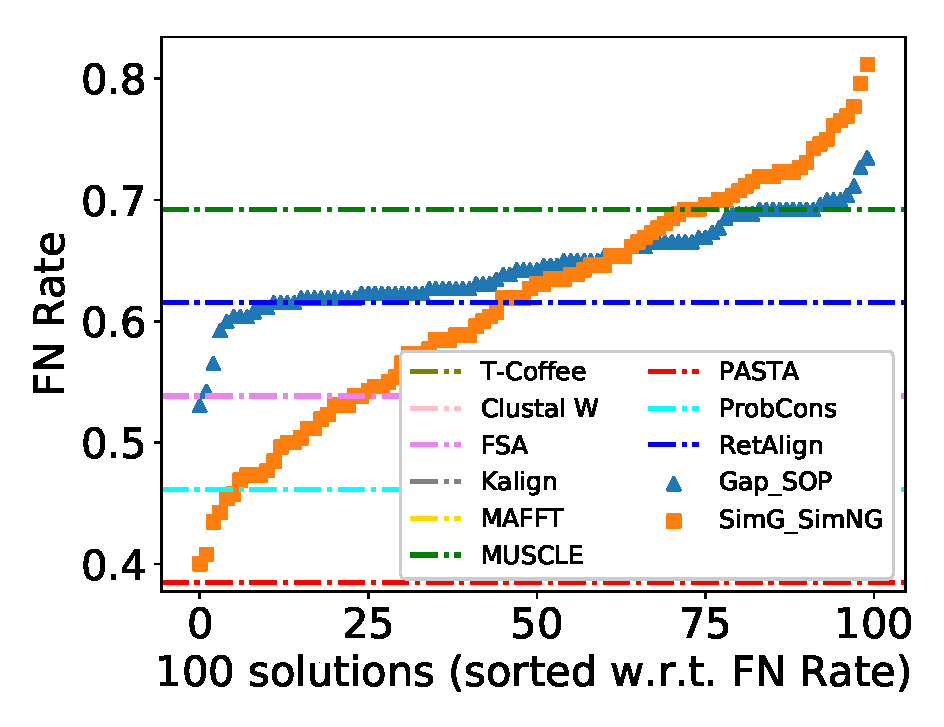
\includegraphics[width=\columnwidth]{Figure/summary/precomputedInit/Balibase/BB20001_fnrate_density_single_run}
			\caption{BB20001}
			%\label{fig:con_pr09}
		\end{subfigure}	
		\begin{subfigure}{0.22\textwidth}
			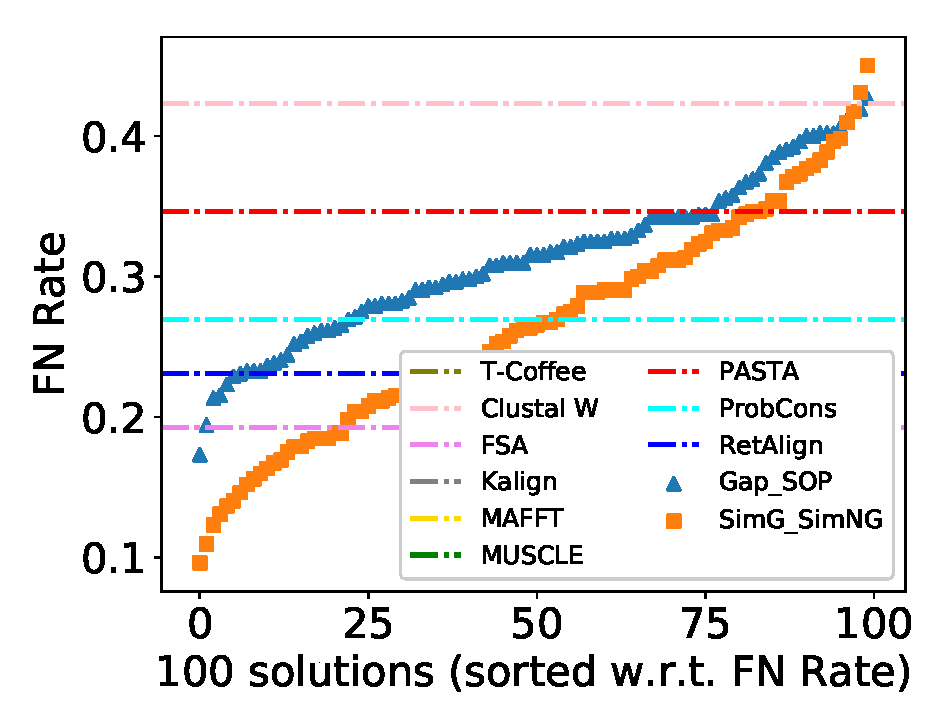
\includegraphics[width=\columnwidth]{Figure/summary/precomputedInit/Balibase/BB20010_fnrate_density_single_run}
			\caption{BB20010}
			%\label{fig:con_pr09}
		\end{subfigure}
		\begin{subfigure}{0.22\textwidth}
			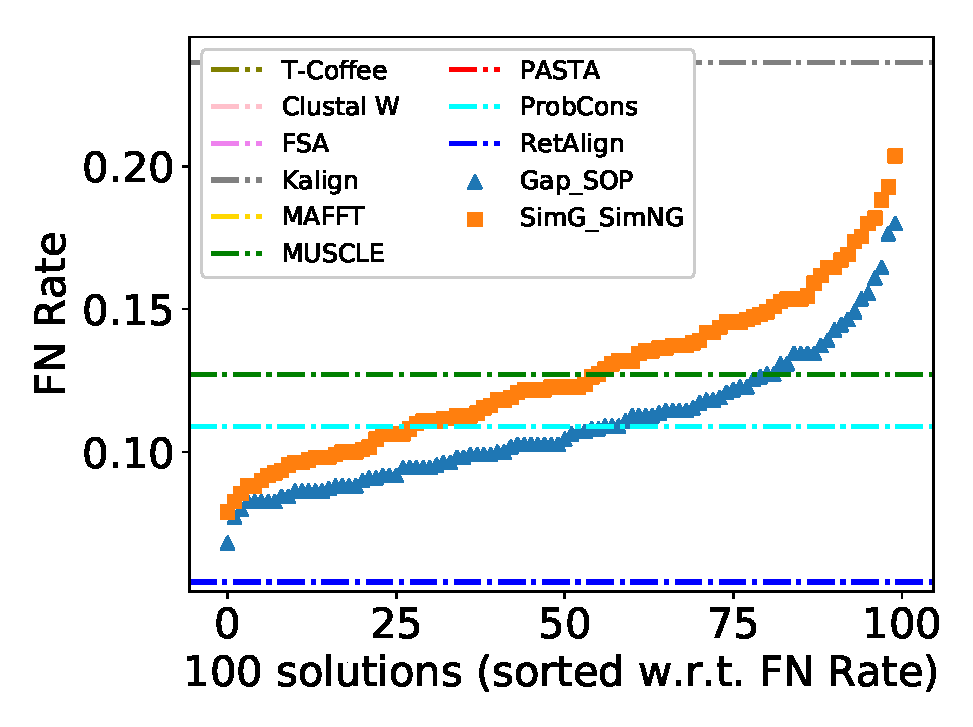
\includegraphics[width=\columnwidth]{Figure/summary/precomputedInit/Balibase/BB20022_fnrate_density_single_run}
			\caption{BB20022}
			%\label{fig:con_pr09}
		\end{subfigure}
		\begin{subfigure}{0.22\textwidth}
			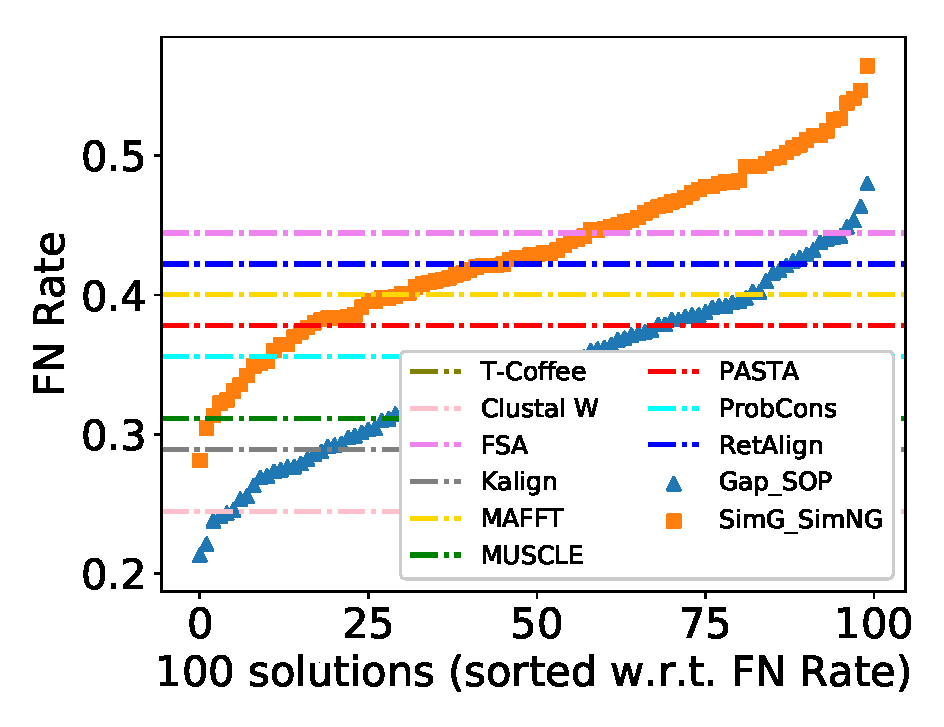
\includegraphics[width=\columnwidth]{Figure/summary/precomputedInit/Balibase/BB20033_fnrate_density_single_run}
			\caption{BB20033}
			%\label{fig:con_pr09}
		\end{subfigure}
		\begin{subfigure}{0.22\textwidth}
			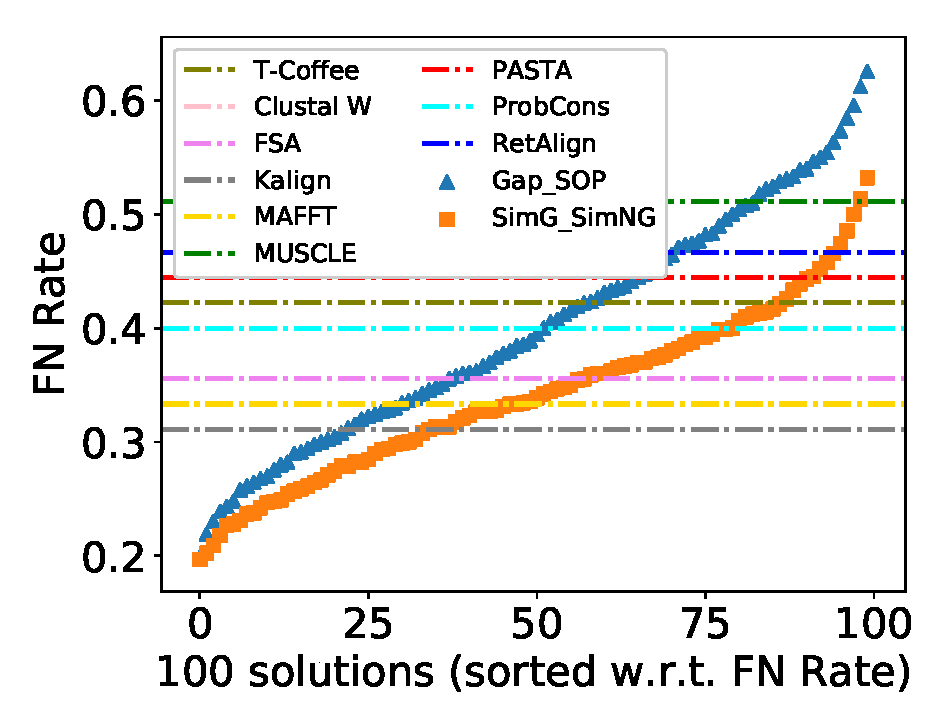
\includegraphics[width=\columnwidth]{Figure/summary/precomputedInit/Balibase/BB20041_fnrate_density_single_run}
			\caption{BB20041}
			%\label{fig:con_pr09}
		\end{subfigure}
		\begin{subfigure}{0.22\textwidth}
			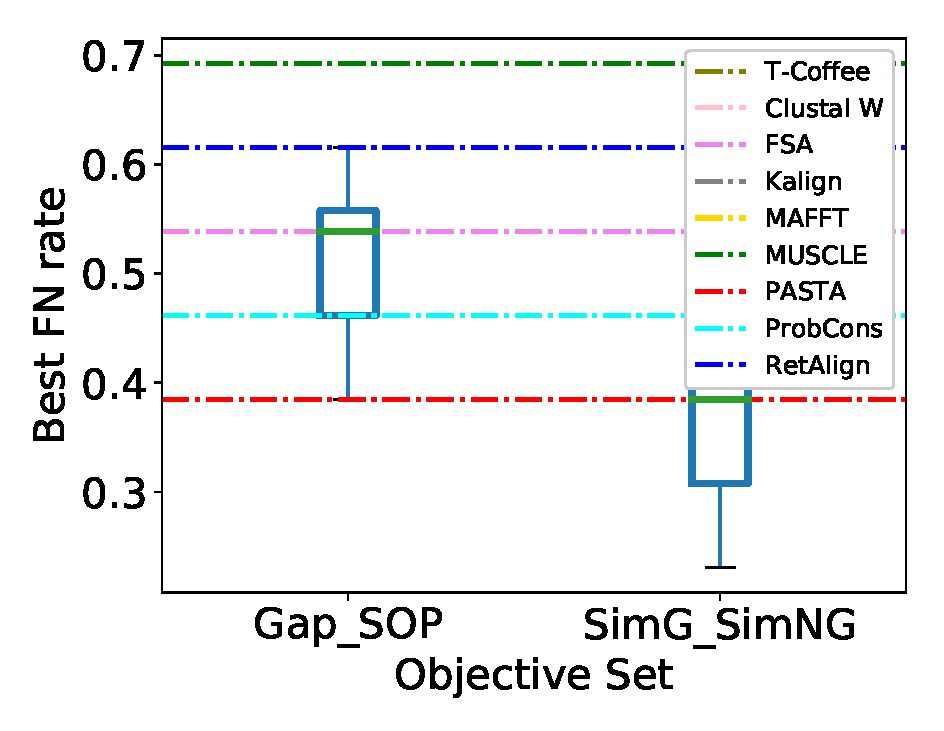
\includegraphics[width=\columnwidth]{Figure/summary/precomputedInit/Balibase/BB20001_objset_fnrate_rank}
			\caption{BB20001}
			%\label{fig:con_pr09}
		\end{subfigure}	
		\begin{subfigure}{0.22\textwidth}
			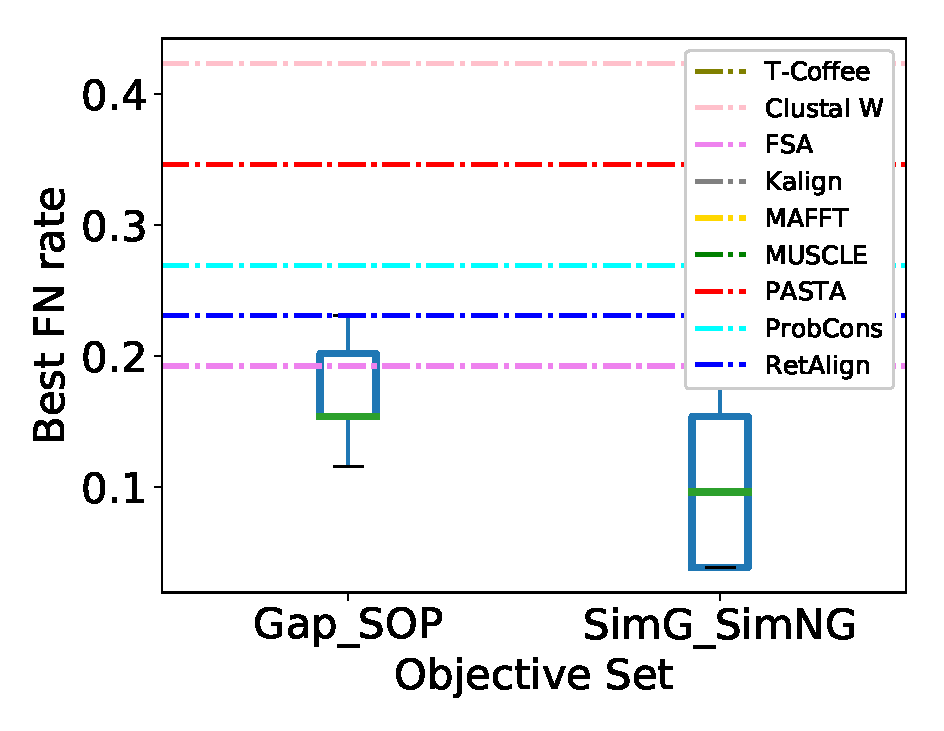
\includegraphics[width=\columnwidth]{Figure/summary/precomputedInit/Balibase/BB20010_objset_fnrate_rank}
			\caption{BB20010}
			%\label{fig:con_pr09}
		\end{subfigure}
		\begin{subfigure}{0.22\textwidth}
			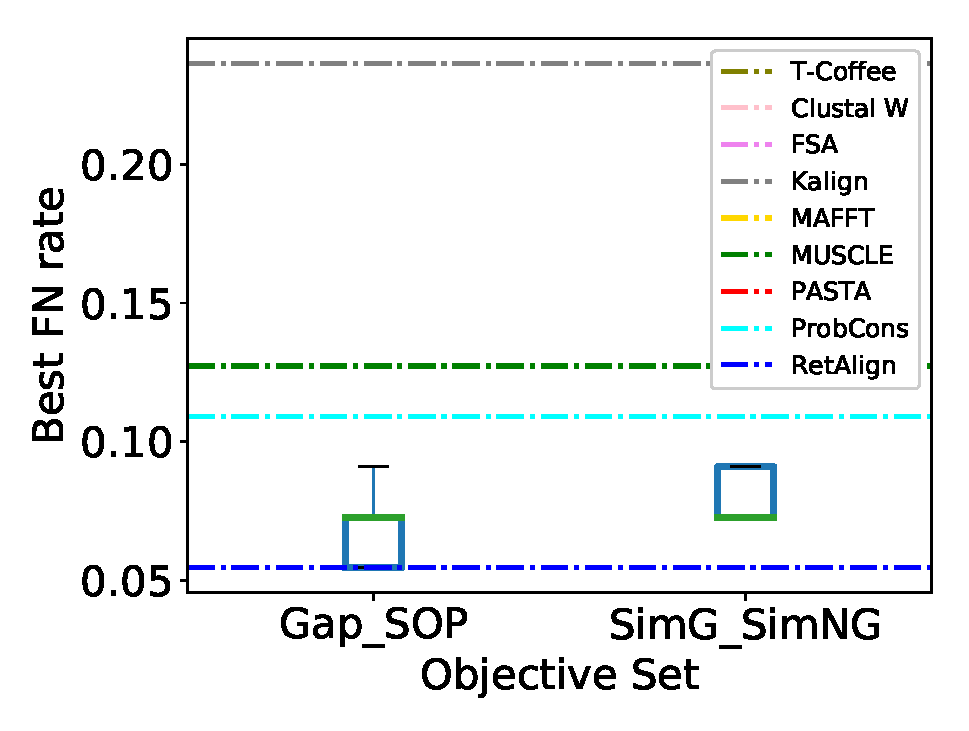
\includegraphics[width=\columnwidth]{Figure/summary/precomputedInit/Balibase/BB20022_objset_fnrate_rank}
			\caption{BB20022}
			%\label{fig:con_pr09}
		\end{subfigure}
		\begin{subfigure}{0.22\textwidth}
			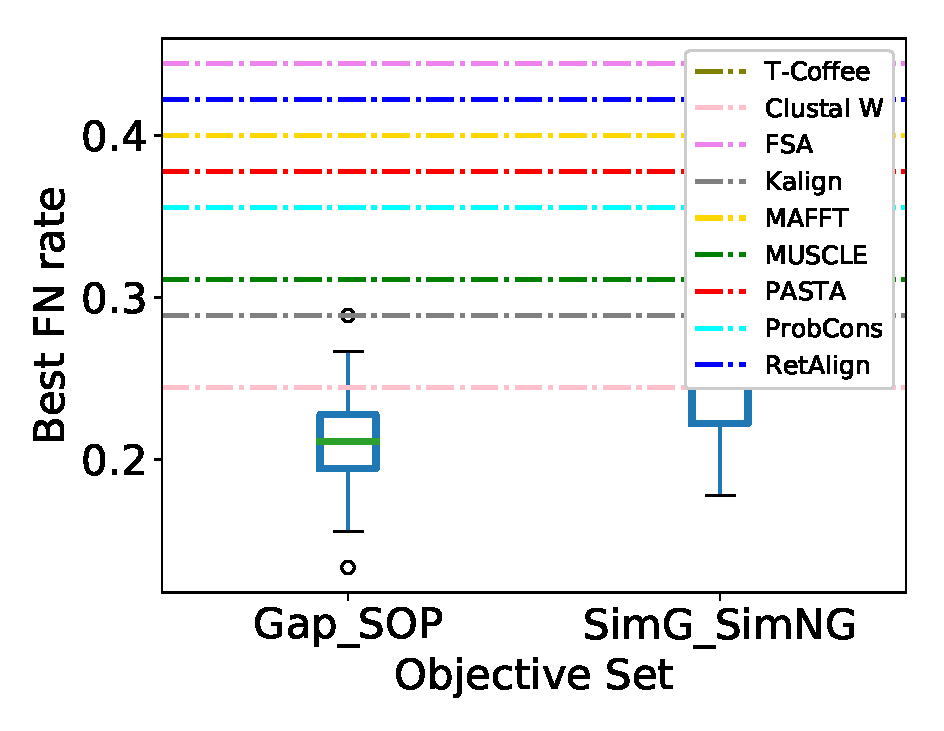
\includegraphics[width=\columnwidth]{Figure/summary/precomputedInit/Balibase/BB20033_objset_fnrate_rank}
			\caption{BB20033}
			%\label{fig:con_pr09}
		\end{subfigure}
		\begin{subfigure}{0.22\textwidth}
			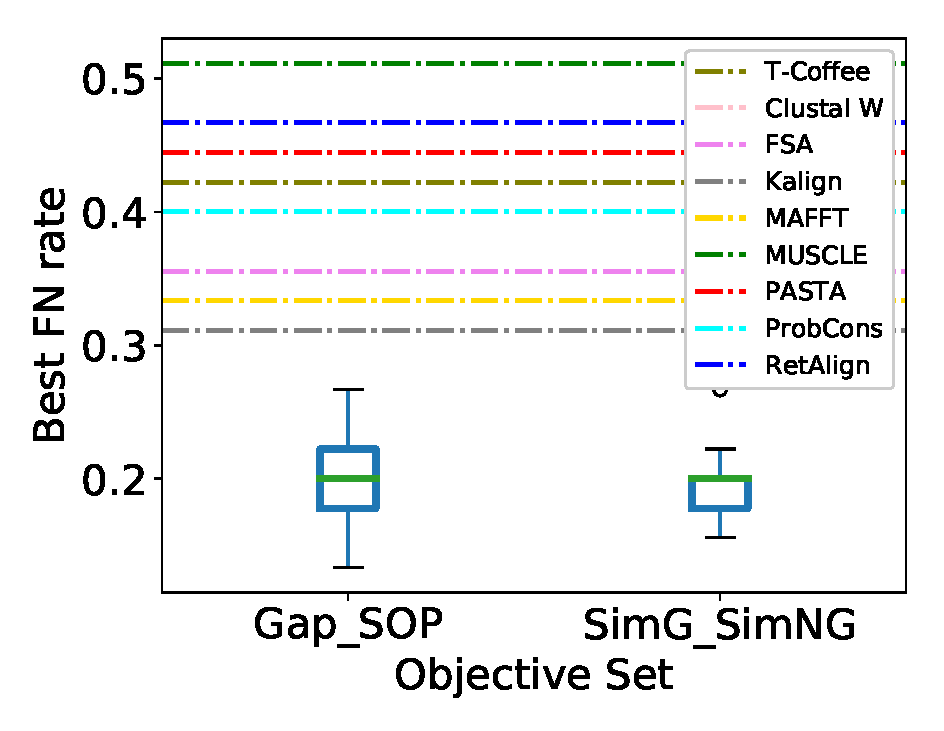
\includegraphics[width=\columnwidth]{Figure/summary/precomputedInit/Balibase/BB20041_objset_fnrate_rank}
			\caption{BB20041}
			%\label{fig:con_pr09}
		\end{subfigure}
		\end{adjustwidth}
		\caption[FN rate results on RV20]{\underline{RV20:} Top panel (part (a) - (d)) shows the FN rate of 100 final solutions averaged over 20 runs. At first, we sort the FN rates of each solution set. Then we average the FN rates at each sorted position of all the sets. Bottom panel (part (e) - (h)) shows the distribution of the best FN rates collected from all runs. In each figure, the horizontal lines show the performance of the state-of-the-art tools.}
		\label{fig:rv20_fn_rate}

\end{figure*}


\begin{figure*}[!htbp]
	\centering
	\begin{adjustwidth}{-1.5cm}{-1cm}
		\begin{subfigure}{0.22\textwidth}
			\includegraphics[width=\columnwidth]{Figure/summary/precomputedInit/Balibase/BB20001_tc_density_single_run_2}
			\caption{BB20001}
			%\label{fig:con_pr09}
		\end{subfigure}	
		\begin{subfigure}{0.22\textwidth}
			\includegraphics[width=\columnwidth]{Figure/summary/precomputedInit/Balibase/BB20010_tc_density_single_run_2}
			\caption{BB20010}
			%\label{fig:con_pr09}
		\end{subfigure}
		\begin{subfigure}{0.22\textwidth}
			\includegraphics[width=\columnwidth]{Figure/summary/precomputedInit/Balibase/BB20022_tc_density_single_run_2}
			\caption{BB20022}
			%\label{fig:con_pr09}
		\end{subfigure}
		\begin{subfigure}{0.22\textwidth}
			\includegraphics[width=\columnwidth]{Figure/summary/precomputedInit/Balibase/BB20033_tc_density_single_run_2}
			\caption{BB20033}
			%\label{fig:con_pr09}
		\end{subfigure}
		\begin{subfigure}{0.22\textwidth}
			\includegraphics[width=\columnwidth]{Figure/summary/precomputedInit/Balibase/BB20041_tc_density_single_run_2}
			\caption{BB20041}
			%\label{fig:con_pr09}
		\end{subfigure}
		\begin{subfigure}{0.22\textwidth}
			\includegraphics[width=\columnwidth]{Figure/summary/precomputedInit/Balibase/BB20001_objset_tc_rank_2}
			\caption{BB20001}
			%\label{fig:con_pr09}
		\end{subfigure}	
		\begin{subfigure}{0.22\textwidth}
			\includegraphics[width=\columnwidth]{Figure/summary/precomputedInit/Balibase/BB20010_objset_tc_rank_2}
			\caption{BB20010}
			%\label{fig:con_pr09}
		\end{subfigure}
		\begin{subfigure}{0.22\textwidth}
			\includegraphics[width=\columnwidth]{Figure/summary/precomputedInit/Balibase/BB20022_objset_tc_rank_2}
			\caption{BB20022}
			%\label{fig:con_pr09}
		\end{subfigure}
		\begin{subfigure}{0.22\textwidth}
			\includegraphics[width=\columnwidth]{Figure/summary/precomputedInit/Balibase/BB20033_objset_tc_rank_2}
			\caption{BB20033}
			%\label{fig:con_pr09}
		\end{subfigure}
		\begin{subfigure}{0.22\textwidth}
			\includegraphics[width=\columnwidth]{Figure/summary/precomputedInit/Balibase/BB20041_objset_tc_rank_2}
			\caption{BB20041}
			%\label{fig:con_pr09}
		\end{subfigure}
		\end{adjustwidth}
		\caption[TC score results on RV20]{\underline{RV20:} Top panel (part (a) - (e)) shows the TC score of 100 final solutions averaged over 20 runs. At first, we sort the TC scores of each solution set. Then we average the TC scores at each sorted position of all the sets. Bottom panel (part (f) - (j)) shows the distribution of the best TC scores collected from all runs. In each figure, the horizontal lines show the performance of the state-of-the-art tools.}
		\label{fig:rv20_tc}

\end{figure*}

\begin{figure*}[!htbp]
	\centering
	\begin{adjustwidth}{-1.5cm}{-1cm}
		\begin{subfigure}{0.22\textwidth}
			\includegraphics[width=\columnwidth]{Figure/summary/precomputedInit/Balibase/BB20001_pairs_density_single_run_2}
			\caption{BB20001}
			%\label{fig:con_pr09}
		\end{subfigure}	
		\begin{subfigure}{0.22\textwidth}
			\includegraphics[width=\columnwidth]{Figure/summary/precomputedInit/Balibase/BB20010_pairs_density_single_run_2}
			\caption{BB20010}
			%\label{fig:con_pr09}
		\end{subfigure}
		\begin{subfigure}{0.22\textwidth}
			\includegraphics[width=\columnwidth]{Figure/summary/precomputedInit/Balibase/BB20022_pairs_density_single_run_2}
			\caption{BB20022}
			%\label{fig:con_pr09}
		\end{subfigure}
		\begin{subfigure}{0.22\textwidth}
			\includegraphics[width=\columnwidth]{Figure/summary/precomputedInit/Balibase/BB20033_pairs_density_single_run_2}
			\caption{BB20033}
			%\label{fig:con_pr09}
		\end{subfigure}
		\begin{subfigure}{0.22\textwidth}
			\includegraphics[width=\columnwidth]{Figure/summary/precomputedInit/Balibase/BB20041_pairs_density_single_run_2}
			\caption{BB20041}
			%\label{fig:con_pr09}
		\end{subfigure}
		\begin{subfigure}{0.22\textwidth}
			\includegraphics[width=\columnwidth]{Figure/summary/precomputedInit/Balibase/BB20001_objset_pairs_rank_2}
			\caption{BB20001}
			%\label{fig:con_pr09}
		\end{subfigure}	
		\begin{subfigure}{0.22\textwidth}
			\includegraphics[width=\columnwidth]{Figure/summary/precomputedInit/Balibase/BB20010_objset_pairs_rank_2}
			\caption{BB20010}
			%\label{fig:con_pr09}
		\end{subfigure}
		\begin{subfigure}{0.22\textwidth}
			\includegraphics[width=\columnwidth]{Figure/summary/precomputedInit/Balibase/BB20022_objset_pairs_rank_2}
			\caption{BB20022}
			%\label{fig:con_pr09}
		\end{subfigure}
		\begin{subfigure}{0.22\textwidth}
			\includegraphics[width=\columnwidth]{Figure/summary/precomputedInit/Balibase/BB20033_objset_pairs_rank_2}
			\caption{BB20033}
			%\label{fig:con_pr09}
		\end{subfigure}
		\begin{subfigure}{0.22\textwidth}
			\includegraphics[width=\columnwidth]{Figure/summary/precomputedInit/Balibase/BB20041_objset_pairs_rank_2}
			\caption{BB20041}
			%\label{fig:con_pr09}
		\end{subfigure}
		\end{adjustwidth}
		\caption[SP score results on RV20]{\underline{RV20:} Top panel (part (a) - (e)) shows the SP score of 100 final solutions averaged over 20 runs. At first, we sort the SP scores of each solution set. Then we average the SP scores at each sorted position of all the sets. Bottom panel (part (f) - (j)) shows the distribution of the best SP scores collected from all runs. In each figure, the horizontal lines show the performance of the state-of-the-art tools.}
		\label{fig:rv20_sp}

\end{figure*}


\begin{figure*}[!htbp]
	\centering
	\begin{adjustwidth}{-1.5cm}{-1cm}
		\begin{subfigure}{0.22\textwidth}
			\includegraphics[width=\columnwidth]{Figure/summary/precomputedInit/Balibase/BB20001_fnrate_vs_tc_2}
			\caption{BB20001}
			%\label{fig:con_pr09}
		\end{subfigure}	
		\begin{subfigure}{0.22\textwidth}
			\includegraphics[width=\columnwidth]{Figure/summary/precomputedInit/Balibase/BB20010_fnrate_vs_tc_2}
			\caption{BB20010}
			%\label{fig:con_pr09}
		\end{subfigure}
		\begin{subfigure}{0.22\textwidth}
			\includegraphics[width=\columnwidth]{Figure/summary/precomputedInit/Balibase/BB20022_fnrate_vs_tc_2}
			\caption{BB20022}
			%\label{fig:con_pr09}
		\end{subfigure}
		\begin{subfigure}{0.22\textwidth}
			\includegraphics[width=\columnwidth]{Figure/summary/precomputedInit/Balibase/BB20033_fnrate_vs_tc_2}
			\caption{BB20033}
			%\label{fig:con_pr09}
		\end{subfigure}	
		\begin{subfigure}{0.22\textwidth}
			\includegraphics[width=\columnwidth]{Figure/summary/precomputedInit/Balibase/BB20041_fnrate_vs_tc_2}
			\caption{BB20041}
			%\label{fig:con_pr09}
		\end{subfigure}
		%%%%%%%%%%
		\begin{subfigure}{0.22\textwidth}
			\includegraphics[width=\columnwidth]{Figure/summary/precomputedInit/Balibase/BB20001_fnrate_vs_sp_2}
			\caption{BB20001}
			%\label{fig:con_pr09}
		\end{subfigure}	
		\begin{subfigure}{0.22\textwidth}
			\includegraphics[width=\columnwidth]{Figure/summary/precomputedInit/Balibase/BB20010_fnrate_vs_sp_2}
			\caption{BB20010}
			%\label{fig:con_pr09}
		\end{subfigure}
		\begin{subfigure}{0.22\textwidth}
			\includegraphics[width=\columnwidth]{Figure/summary/precomputedInit/Balibase/BB20022_fnrate_vs_sp_2}
			\caption{BB20022}
			%\label{fig:con_pr09}
		\end{subfigure}
		\begin{subfigure}{0.22\textwidth}
			\includegraphics[width=\columnwidth]{Figure/summary/precomputedInit/Balibase/BB20033_fnrate_vs_sp_2}
			\caption{BB20033}
			%\label{fig:con_pr09}
		\end{subfigure}	
		\begin{subfigure}{0.22\textwidth}
			\includegraphics[width=\columnwidth]{Figure/summary/precomputedInit/Balibase/BB20041_fnrate_vs_sp_2}
			\caption{BB20041}
			%\label{fig:con_pr09}
		\end{subfigure}
		\end{adjustwidth}
		\caption[FN rate vs TC score on RV20]{\underline{RV20:} Top panel (part (a) - (e)) shows the relationship between FN rate and TC score for different alignments. And bottom panel (part (f) - (j)) shows the relationship between FN rate and SP score. The horizontal lines mark the FN rates achieved by the state-of-the-art tools.}
		\label{fig:rv20_fnrate_vs_tc}

\end{figure*}
%############################# RV30
\begin{figure*}[!htbp]
	
	\begin{adjustwidth}{-1cm}{-1cm}
		\centering
		\begin{subfigure}{0.22\textwidth}
			\includegraphics[width=\columnwidth]{Figure/summary/precomputedInit/Balibase/BB30002_fnrate_density_single_run}
			\caption{BB30002}
			%\label{fig:con_pr09}
		\end{subfigure}	
		\begin{subfigure}{0.22\textwidth}
			\includegraphics[width=\columnwidth]{Figure/summary/precomputedInit/Balibase/BB30008_fnrate_density_single_run}
			\caption{BB30008}
			%\label{fig:con_pr09}
		\end{subfigure}
		\begin{subfigure}{0.22\textwidth}
			\includegraphics[width=\columnwidth]{Figure/summary/precomputedInit/Balibase/BB30015_fnrate_density_single_run}
			\caption{BB30015}
			%\label{fig:con_pr09}
		\end{subfigure}
		\begin{subfigure}{0.22\textwidth}
			\includegraphics[width=\columnwidth]{Figure/summary/precomputedInit/Balibase/BB30022_fnrate_density_single_run}
			\caption{BB30022}
			%\label{fig:con_pr09}
		\end{subfigure}
		\begin{subfigure}{0.22\textwidth}
			\includegraphics[width=\columnwidth]{Figure/summary/precomputedInit/Balibase/BB30002_objset_fnrate_rank}
			\caption{BB30002}
			%\label{fig:con_pr09}
		\end{subfigure}
		\begin{subfigure}{0.22\textwidth}
			\includegraphics[width=\columnwidth]{Figure/summary/precomputedInit/Balibase/BB30008_objset_fnrate_rank}
			\caption{BB30008}
			%\label{fig:con_pr09}
		\end{subfigure}		
		\begin{subfigure}{0.22\textwidth}
			\includegraphics[width=\columnwidth]{Figure/summary/precomputedInit/Balibase/BB30015_objset_fnrate_rank}
			\caption{BB30015}
			%\label{fig:con_pr09}
		\end{subfigure}
		\begin{subfigure}{0.22\textwidth}
			\includegraphics[width=\columnwidth]{Figure/summary/precomputedInit/Balibase/BB30022_objset_fnrate_rank}
			\caption{BB30022}
			%\label{fig:con_pr09}
		\end{subfigure}
		\end{adjustwidth}
		\caption[FN rate results on RV30]{\underline{RV30:} Top panel (part (a) - (d)) shows the FN rate of 100 final solutions averaged over 20 runs. At first, we sort the FN rates of each solution set. Then we average the FN rates at each sorted position of all the sets. Bottom panel (part (e) - (h)) shows the distribution of the best FN rates collected from all runs. In each figure, the horizontal lines show the performance of the state-of-the-art tools.}
		\label{fig:rv30_fn_rate}

\end{figure*}



\begin{figure*}[!htbp]
	
	\begin{adjustwidth}{-1cm}{-1cm}
		\centering
		\begin{subfigure}{0.22\textwidth}
			\includegraphics[width=\columnwidth]{Figure/summary/precomputedInit/Balibase/BB30002_tc_density_single_run_2}
			\caption{BB30002}
			%\label{fig:con_pr09}
		\end{subfigure}	
		\begin{subfigure}{0.22\textwidth}
			\includegraphics[width=\columnwidth]{Figure/summary/precomputedInit/Balibase/BB30008_tc_density_single_run_2}
			\caption{BB30008}
			%\label{fig:con_pr09}
		\end{subfigure}
		\begin{subfigure}{0.22\textwidth}
			\includegraphics[width=\columnwidth]{Figure/summary/precomputedInit/Balibase/BB30015_tc_density_single_run_2}
			\caption{BB30015}
			%\label{fig:con_pr09}
		\end{subfigure}
		\begin{subfigure}{0.22\textwidth}
			\includegraphics[width=\columnwidth]{Figure/summary/precomputedInit/Balibase/BB30022_tc_density_single_run_2}
			\caption{BB30022}
			%\label{fig:con_pr09}
		\end{subfigure}
		\begin{subfigure}{0.22\textwidth}
			\includegraphics[width=\columnwidth]{Figure/summary/precomputedInit/Balibase/BB30002_objset_tc_rank_2}
			\caption{BB30002}
			%\label{fig:con_pr09}
		\end{subfigure}	
		\begin{subfigure}{0.22\textwidth}
			\includegraphics[width=\columnwidth]{Figure/summary/precomputedInit/Balibase/BB30008_objset_tc_rank_2}
			\caption{BB30008}
			%\label{fig:con_pr09}
		\end{subfigure}
		\begin{subfigure}{0.22\textwidth}
			\includegraphics[width=\columnwidth]{Figure/summary/precomputedInit/Balibase/BB30015_objset_tc_rank_2}
			\caption{BB30015}
			%\label{fig:con_pr09}
		\end{subfigure}
		\begin{subfigure}{0.22\textwidth}
			\includegraphics[width=\columnwidth]{Figure/summary/precomputedInit/Balibase/BB30022_objset_tc_rank_2}
			\caption{BB30022}
			%\label{fig:con_pr09}
		\end{subfigure}
		\end{adjustwidth}
		\caption[TC score results on RV30]{\underline{RV30:} Top panel (part (a) - (d)) shows the TC score of 100 final solutions averaged over 20 runs. At first, we sort the TC scores of each solution set. Then we average the TC scores at each sorted position of all the sets. Bottom panel (part (e) - (h)) shows the distribution of the best TC scores collected from all runs. In each figure, the horizontal lines show the performance of the state-of-the-art tools.}
		\label{fig:rv30_tc}

\end{figure*}

\begin{figure*}[!htbp]
	
	\begin{adjustwidth}{-1cm}{-1cm}
		\centering
		\begin{subfigure}{0.22\textwidth}
			\includegraphics[width=\columnwidth]{Figure/summary/precomputedInit/Balibase/BB30002_pairs_density_single_run_2}
			\caption{BB30002}
			%\label{fig:con_pr09}
		\end{subfigure}	
		\begin{subfigure}{0.22\textwidth}
			\includegraphics[width=\columnwidth]{Figure/summary/precomputedInit/Balibase/BB30008_pairs_density_single_run_2}
			\caption{BB30008}
			%\label{fig:con_pr09}
		\end{subfigure}
		\begin{subfigure}{0.22\textwidth}
			\includegraphics[width=\columnwidth]{Figure/summary/precomputedInit/Balibase/BB30015_pairs_density_single_run_2}
			\caption{BB30015}
			%\label{fig:con_pr09}
		\end{subfigure}
		\begin{subfigure}{0.22\textwidth}
			\includegraphics[width=\columnwidth]{Figure/summary/precomputedInit/Balibase/BB30022_pairs_density_single_run_2}
			\caption{BB30022}
			%\label{fig:con_pr09}
		\end{subfigure}
		\begin{subfigure}{0.22\textwidth}
			\includegraphics[width=\columnwidth]{Figure/summary/precomputedInit/Balibase/BB30002_objset_pairs_rank_2}
			\caption{BB30002}
			%\label{fig:con_pr09}
		\end{subfigure}	
		\begin{subfigure}{0.22\textwidth}
			\includegraphics[width=\columnwidth]{Figure/summary/precomputedInit/Balibase/BB30008_objset_pairs_rank_2}
			\caption{BB30008}
			%\label{fig:con_pr09}
		\end{subfigure}
		\begin{subfigure}{0.22\textwidth}
			\includegraphics[width=\columnwidth]{Figure/summary/precomputedInit/Balibase/BB30015_objset_pairs_rank_2}
			\caption{BB30015}
			%\label{fig:con_pr09}
		\end{subfigure}
		\begin{subfigure}{0.22\textwidth}
			\includegraphics[width=\columnwidth]{Figure/summary/precomputedInit/Balibase/BB30022_objset_pairs_rank_2}
			\caption{BB30022}
			%\label{fig:con_pr09}
		\end{subfigure}
		\end{adjustwidth}
		\caption[SP score results on RV30]{\underline{RV30:} Top panel (part (a) - (d)) shows the SP score of 100 final solutions averaged over 20 runs. At first, we sort the SP scores of each solution set. Then we average the SP scores at each sorted position of all the sets. Bottom panel (part (e) - (h)) shows the distribution of the best SP scores collected from all runs. In each figure, the horizontal lines show the performance of the state-of-the-art tools.}
		\label{fig:rv30_sp}

\end{figure*}


\begin{figure*}[!htbp]
	
	\begin{adjustwidth}{-1cm}{-1cm}
		\centering
		\begin{subfigure}{0.22\textwidth}
			\includegraphics[width=\columnwidth]{Figure/summary/precomputedInit/Balibase/BB30002_fnrate_vs_tc_2}
			\caption{BB30002}
			%\label{fig:con_pr09}
		\end{subfigure}	
		\begin{subfigure}{0.22\textwidth}
			\includegraphics[width=\columnwidth]{Figure/summary/precomputedInit/Balibase/BB30008_fnrate_vs_tc_2}
			\caption{BB30008}
			%\label{fig:con_pr09}
		\end{subfigure}
		\begin{subfigure}{0.22\textwidth}
			\includegraphics[width=\columnwidth]{Figure/summary/precomputedInit/Balibase/BB30015_fnrate_vs_tc_2}
			\caption{BB30015}
			%\label{fig:con_pr09}
		\end{subfigure}
		\begin{subfigure}{0.22\textwidth}
			\includegraphics[width=\columnwidth]{Figure/summary/precomputedInit/Balibase/BB30022_fnrate_vs_tc_2}
			\caption{BB30022}
			%\label{fig:con_pr09}
		\end{subfigure}	
		\begin{subfigure}{0.22\textwidth}
			\includegraphics[width=\columnwidth]{Figure/summary/precomputedInit/Balibase/BB30002_fnrate_vs_sp_2}
			\caption{BB30002}
			%\label{fig:con_pr09}
		\end{subfigure}	
		\begin{subfigure}{0.22\textwidth}
			\includegraphics[width=\columnwidth]{Figure/summary/precomputedInit/Balibase/BB30008_fnrate_vs_sp_2}
			\caption{BB30008}
			%\label{fig:con_pr09}
		\end{subfigure}
		\begin{subfigure}{0.22\textwidth}
			\includegraphics[width=\columnwidth]{Figure/summary/precomputedInit/Balibase/BB30015_fnrate_vs_sp_2}
			\caption{BB30015}
			%\label{fig:con_pr09}
		\end{subfigure}
		\begin{subfigure}{0.22\textwidth}
			\includegraphics[width=\columnwidth]{Figure/summary/precomputedInit/Balibase/BB30022_fnrate_vs_sp_2}
			\caption{BB30022}
			%\label{fig:con_pr09}
		\end{subfigure}	
		\end{adjustwidth}
		\caption[FN rate vs TC score on RV30]{\underline{RV30:} Top panel (part (a) - (d)) shows the relationship between FN rate and TC score for different alignments. And bottom panel (part (e) - (h)) shows the relationship between FN rate and SP score. The horizontal lines mark the FN rates achieved by the state-of-the-art tools.}
		\label{fig:rv30_fnrate_vs_tc}

\end{figure*}
%############################# RV40
\begin{figure*}[!htbp]
	\centering
	\begin{adjustwidth}{-1.5cm}{-1cm}
		\begin{subfigure}{0.22\textwidth}
			\includegraphics[width=\columnwidth]{Figure/summary/precomputedInit/Balibase/BB40001_fnrate_density_single_run}
			\caption{BB40001}
			%\label{fig:con_pr09}
		\end{subfigure}	
		\begin{subfigure}{0.22\textwidth}
			\includegraphics[width=\columnwidth]{Figure/summary/precomputedInit/Balibase/BB40013_fnrate_density_single_run}
			\caption{BB40013}
			%\label{fig:con_pr09}
		\end{subfigure}
		\begin{subfigure}{0.22\textwidth}
			\includegraphics[width=\columnwidth]{Figure/summary/precomputedInit/Balibase/BB40025_fnrate_density_single_run}
			\caption{BB40025}
			%\label{fig:con_pr09}
		\end{subfigure}
		\begin{subfigure}{0.22\textwidth}
			\includegraphics[width=\columnwidth]{Figure/summary/precomputedInit/Balibase/BB40038_fnrate_density_single_run}
			\caption{BB40038}
			%\label{fig:con_pr09}
		\end{subfigure}
		\begin{subfigure}{0.22\textwidth}
			\includegraphics[width=\columnwidth]{Figure/summary/precomputedInit/Balibase/BB40048_fnrate_density_single_run}
			\caption{BB40048}
			%\label{fig:con_pr09}
		\end{subfigure}
		
		\begin{subfigure}{0.22\textwidth}
			\includegraphics[width=\columnwidth]{Figure/summary/precomputedInit/Balibase/BB40001_objset_fnrate_rank}
			\caption{BB40001}
			%\label{fig:con_pr09}
		\end{subfigure}	
		\begin{subfigure}{0.22\textwidth}
			\includegraphics[width=\columnwidth]{Figure/summary/precomputedInit/Balibase/BB40013_objset_fnrate_rank}
			\caption{BB40013}
			%\label{fig:con_pr09}
		\end{subfigure}
		\begin{subfigure}{0.22\textwidth}
			\includegraphics[width=\columnwidth]{Figure/summary/precomputedInit/Balibase/BB40025_objset_fnrate_rank}
			\caption{BB40025}
			%\label{fig:con_pr09}
		\end{subfigure}
		\begin{subfigure}{0.22\textwidth}
			\includegraphics[width=\columnwidth]{Figure/summary/precomputedInit/Balibase/BB40038_objset_fnrate_rank}
			\caption{BB40038}
			%\label{fig:con_pr09}
		\end{subfigure}
		\begin{subfigure}{0.22\textwidth}
			\includegraphics[width=\columnwidth]{Figure/summary/precomputedInit/Balibase/BB40048_objset_fnrate_rank}
			\caption{BB40048}
			%\label{fig:con_pr09}
		\end{subfigure}
		\end{adjustwidth}
		\caption[FN rate results on RV40]{\underline{RV40:} Top panel (part (a) - (d)) shows the FN rate of 100 final solutions averaged over 20 runs. At first, we sort the FN rates of each solution set. Then we average the FN rates at each sorted position of all the sets. Bottom panel (part (e) - (h)) shows the distribution of the best FN rates collected from all runs. In each figure, the horizontal lines show the performance of the state-of-the-art tools.}
		\label{fig:rv40_fn_rate}

\end{figure*}


\begin{figure*}[!htbp]
	\centering
	\begin{adjustwidth}{-1.5cm}{-1cm}
		\begin{subfigure}{0.22\textwidth}
			\includegraphics[width=\columnwidth]{Figure/summary/precomputedInit/Balibase/BB40001_tc_density_single_run_2}
			\caption{BB40001}
			%\label{fig:con_pr09}
		\end{subfigure}	
		\begin{subfigure}{0.22\textwidth}
			\includegraphics[width=\columnwidth]{Figure/summary/precomputedInit/Balibase/BB40013_tc_density_single_run_2}
			\caption{BB40013}
			%\label{fig:con_pr09}
		\end{subfigure}
		\begin{subfigure}{0.22\textwidth}
			\includegraphics[width=\columnwidth]{Figure/summary/precomputedInit/Balibase/BB40025_tc_density_single_run_2}
			\caption{BB40025}
			%\label{fig:con_pr09}
		\end{subfigure}
		\begin{subfigure}{0.22\textwidth}
			\includegraphics[width=\columnwidth]{Figure/summary/precomputedInit/Balibase/BB40038_tc_density_single_run_2}
			\caption{BB40038}
			%\label{fig:con_pr09}
		\end{subfigure}
		\begin{subfigure}{0.22\textwidth}
			\includegraphics[width=\columnwidth]{Figure/summary/precomputedInit/Balibase/BB40048_tc_density_single_run_2}
			\caption{BB40048}
			%\label{fig:con_pr09}
		\end{subfigure}
		\begin{subfigure}{0.22\textwidth}
			\includegraphics[width=\columnwidth]{Figure/summary/precomputedInit/Balibase/BB40001_objset_tc_rank_2}
			\caption{BB40001}
			%\label{fig:con_pr09}
		\end{subfigure}	
		\begin{subfigure}{0.22\textwidth}
			\includegraphics[width=\columnwidth]{Figure/summary/precomputedInit/Balibase/BB40013_objset_tc_rank_2}
			\caption{BB40013}
			%\label{fig:con_pr09}
		\end{subfigure}
		\begin{subfigure}{0.22\textwidth}
			\includegraphics[width=\columnwidth]{Figure/summary/precomputedInit/Balibase/BB40025_objset_tc_rank_2}
			\caption{BB40025}
			%\label{fig:con_pr09}
		\end{subfigure}
		\begin{subfigure}{0.22\textwidth}
			\includegraphics[width=\columnwidth]{Figure/summary/precomputedInit/Balibase/BB40038_objset_tc_rank_2}
			\caption{BB40038}
			%\label{fig:con_pr09}
		\end{subfigure}
		\begin{subfigure}{0.22\textwidth}
			\includegraphics[width=\columnwidth]{Figure/summary/precomputedInit/Balibase/BB40048_objset_tc_rank_2}
			\caption{BB40048}
			%\label{fig:con_pr09}
		\end{subfigure}
		\end{adjustwidth}
		\caption[TC score results on RV40]{\underline{RV40:} Top panel (part (a) - (e)) shows the TC score of 100 final solutions averaged over 20 runs. At first, we sort the TC scores of each solution set. Then we average the TC scores at each sorted position of all the sets. Bottom panel (part (f) - (j)) shows the distribution of the best TC scores collected from all runs. In each figure, the horizontal lines show the performance of the state-of-the-art tools.}
		\label{fig:rv40_tc}

\end{figure*}


\begin{figure*}[!htbp]
	\centering
	\begin{adjustwidth}{-1.5cm}{-1cm}
		\begin{subfigure}{0.22\textwidth}
			\includegraphics[width=\columnwidth]{Figure/summary/precomputedInit/Balibase/BB40001_pairs_density_single_run_2}
			\caption{BB40001}
			%\label{fig:con_pr09}
		\end{subfigure}	
		\begin{subfigure}{0.22\textwidth}
			\includegraphics[width=\columnwidth]{Figure/summary/precomputedInit/Balibase/BB40013_pairs_density_single_run_2}
			\caption{BB40013}
			%\label{fig:con_pr09}
		\end{subfigure}
		\begin{subfigure}{0.22\textwidth}
			\includegraphics[width=\columnwidth]{Figure/summary/precomputedInit/Balibase/BB40025_pairs_density_single_run_2}
			\caption{BB40025}
			%\label{fig:con_pr09}
		\end{subfigure}
		\begin{subfigure}{0.22\textwidth}
			\includegraphics[width=\columnwidth]{Figure/summary/precomputedInit/Balibase/BB40038_pairs_density_single_run_2}
			\caption{BB40038}
			%\label{fig:con_pr09}
		\end{subfigure}
		\begin{subfigure}{0.22\textwidth}
			\includegraphics[width=\columnwidth]{Figure/summary/precomputedInit/Balibase/BB40048_pairs_density_single_run_2}
			\caption{BB40048}
			%\label{fig:con_pr09}
		\end{subfigure}
		
		\begin{subfigure}{0.22\textwidth}
			\includegraphics[width=\columnwidth]{Figure/summary/precomputedInit/Balibase/BB40001_objset_pairs_rank_2}
			\caption{BB40001}
			%\label{fig:con_pr09}
		\end{subfigure}	
		\begin{subfigure}{0.22\textwidth}
			\includegraphics[width=\columnwidth]{Figure/summary/precomputedInit/Balibase/BB40013_objset_pairs_rank_2}
			\caption{BB40013}
			%\label{fig:con_pr09}
		\end{subfigure}
		\begin{subfigure}{0.22\textwidth}
			\includegraphics[width=\columnwidth]{Figure/summary/precomputedInit/Balibase/BB40025_objset_pairs_rank_2}
			\caption{BB40025}
			%\label{fig:con_pr09}
		\end{subfigure}
		\begin{subfigure}{0.22\textwidth}
			\includegraphics[width=\columnwidth]{Figure/summary/precomputedInit/Balibase/BB40038_objset_pairs_rank_2}
			\caption{BB40038}
			%\label{fig:con_pr09}
		\end{subfigure}
		\begin{subfigure}{0.22\textwidth}
			\includegraphics[width=\columnwidth]{Figure/summary/precomputedInit/Balibase/BB40048_objset_pairs_rank_2}
			\caption{BB40048}
			%\label{fig:con_pr09}
		\end{subfigure}
		\end{adjustwidth}
		\caption[SP score results on RV40]{\underline{RV40:} Top panel (part (a) - (e)) shows the SP score of 100 final solutions averaged over 20 runs. At first, we sort the SP scores of each solution set. Then we average the SP scores at each sorted position of all the sets. Bottom panel (part (f) - (j)) shows the distribution of the best SP scores collected from all runs. In each figure, the horizontal lines show the performance of the state-of-the-art tools.}
		\label{fig:rv40_sp}

\end{figure*}

\begin{figure*}[!htbp]
	\centering
	\begin{adjustwidth}{-1.5cm}{-1cm}
		\begin{subfigure}{0.22\textwidth}
			\includegraphics[width=\columnwidth]{Figure/summary/precomputedInit/Balibase/BB40001_fnrate_vs_tc_2}
			\caption{BB40001}
			%\label{fig:con_pr09}
		\end{subfigure}	
		\begin{subfigure}{0.22\textwidth}
			\includegraphics[width=\columnwidth]{Figure/summary/precomputedInit/Balibase/BB40013_fnrate_vs_tc_2}
			\caption{BB40013}
			%\label{fig:con_pr09}
		\end{subfigure}
		\begin{subfigure}{0.22\textwidth}
			\includegraphics[width=\columnwidth]{Figure/summary/precomputedInit/Balibase/BB40025_fnrate_vs_tc_2}
			\caption{BB40025}
			%\label{fig:con_pr09}
		\end{subfigure}
		\begin{subfigure}{0.22\textwidth}
			\includegraphics[width=\columnwidth]{Figure/summary/precomputedInit/Balibase/BB40038_fnrate_vs_tc_2}
			\caption{BB40038}
			%\label{fig:con_pr09}
		\end{subfigure}	
		\begin{subfigure}{0.22\textwidth}
			\includegraphics[width=\columnwidth]{Figure/summary/precomputedInit/Balibase/BB40048_fnrate_vs_tc_2}
			\caption{BB40048}
			%\label{fig:con_pr09}
		\end{subfigure}
		\begin{subfigure}{0.22\textwidth}
			\includegraphics[width=\columnwidth]{Figure/summary/precomputedInit/Balibase/BB40001_fnrate_vs_sp_2}
			\caption{BB40001}
			%\label{fig:con_pr09}
		\end{subfigure}	
		\begin{subfigure}{0.22\textwidth}
			\includegraphics[width=\columnwidth]{Figure/summary/precomputedInit/Balibase/BB40013_fnrate_vs_sp_2}
			\caption{BB40013}
			%\label{fig:con_pr09}
		\end{subfigure}
		\begin{subfigure}{0.22\textwidth}
			\includegraphics[width=\columnwidth]{Figure/summary/precomputedInit/Balibase/BB40025_fnrate_vs_sp_2}
			\caption{BB40025}
			%\label{fig:con_pr09}
		\end{subfigure}
		\begin{subfigure}{0.22\textwidth}
			\includegraphics[width=\columnwidth]{Figure/summary/precomputedInit/Balibase/BB40038_fnrate_vs_sp_2}
			\caption{BB40038}
			%\label{fig:con_pr09}
		\end{subfigure}	
		\begin{subfigure}{0.22\textwidth}
			\includegraphics[width=\columnwidth]{Figure/summary/precomputedInit/Balibase/BB40048_fnrate_vs_sp_2}
			\caption{BB40048}
			%\label{fig:con_pr09}
		\end{subfigure}
		\end{adjustwidth}
		\caption[FN rate vs TC score on RV40]{\underline{RV40:} Top panel (part (a) - (e)) shows the relationship between FN rate and TC score for different alignments. And bottom panel (part (f) - (j)) shows the relationship between FN rate and SP score. The horizontal lines mark the FN rates achieved by the state-of-the-art tools.}
		\label{fig:rv40_fnrate_vs_tc}

\end{figure*}
%############################# RV50
\begin{figure*}[!htbp]
	
	\begin{adjustwidth}{-1.5cm}{-1cm}
		\centering
		\begin{subfigure}{0.22\textwidth}
			\includegraphics[width=\columnwidth]{Figure/summary/precomputedInit/Balibase/BB50001_fnrate_density_single_run}
			\caption{BB50001}
			%\label{fig:con_pr09}
		\end{subfigure}	
		\begin{subfigure}{0.22\textwidth}
			\includegraphics[width=\columnwidth]{Figure/summary/precomputedInit/Balibase/BB50005_fnrate_density_single_run}
			\caption{BB50005}
			%\label{fig:con_pr09}
		\end{subfigure}
		\begin{subfigure}{0.22\textwidth}
			\includegraphics[width=\columnwidth]{Figure/summary/precomputedInit/Balibase/BB50010_fnrate_density_single_run}
			\caption{BB50010}
			%\label{fig:con_pr09}
		\end{subfigure}
		\begin{subfigure}{0.22\textwidth}
			\includegraphics[width=\columnwidth]{Figure/summary/precomputedInit/Balibase/BB50016_fnrate_density_single_run}
			\caption{BB50016}
			%\label{fig:con_pr09}
		\end{subfigure}
		
		\begin{subfigure}{0.22\textwidth}
			\includegraphics[width=\columnwidth]{Figure/summary/precomputedInit/Balibase/BB50001_objset_fnrate_rank}
			\caption{BB50001}
			%\label{fig:con_pr09}
		\end{subfigure}
		\begin{subfigure}{0.22\textwidth}
			\includegraphics[width=\columnwidth]{Figure/summary/precomputedInit/Balibase/BB50005_objset_fnrate_rank}
			\caption{BB50005}
			%\label{fig:con_pr09}
		\end{subfigure}		
		\begin{subfigure}{0.22\textwidth}
			\includegraphics[width=\columnwidth]{Figure/summary/precomputedInit/Balibase/BB50010_objset_fnrate_rank}
			\caption{BB50010}
			%\label{fig:con_pr09}
		\end{subfigure}
		\begin{subfigure}{0.22\textwidth}
			\includegraphics[width=\columnwidth]{Figure/summary/precomputedInit/Balibase/BB50016_objset_fnrate_rank}
			\caption{BB50016}
			%\label{fig:con_pr09}
		\end{subfigure}
		\end{adjustwidth}
		\caption[FN rate results on RV50]{\underline{RV50:} Top panel (part (a) - (d)) shows the FN rate of 100 final solutions averaged over 20 runs. At first, we sort the FN rates of each solution set. Then we average the FN rates at each sorted position of all the sets. Bottom panel (part (e) - (h)) shows the distribution of the best FN rates collected from all runs. In each figure, the horizontal lines show the performance of the state-of-the-art tools.}
		\label{fig:rv50_fn_rate}

\end{figure*}


\begin{figure*}[!htbp]
	
	\begin{adjustwidth}{-1.5cm}{-1cm}
		\centering
		\begin{subfigure}{0.22\textwidth}
			\includegraphics[width=\columnwidth]{Figure/summary/precomputedInit/Balibase/BB50001_tc_density_single_run_2}
			\caption{BB50001}
			%\label{fig:con_pr09}
		\end{subfigure}	
		\begin{subfigure}{0.22\textwidth}
			\includegraphics[width=\columnwidth]{Figure/summary/precomputedInit/Balibase/BB50005_tc_density_single_run_2}
			\caption{BB50005}
			%\label{fig:con_pr09}
		\end{subfigure}
		\begin{subfigure}{0.22\textwidth}
			\includegraphics[width=\columnwidth]{Figure/summary/precomputedInit/Balibase/BB50010_tc_density_single_run_2}
			\caption{BB50010}
			%\label{fig:con_pr09}
		\end{subfigure}
		\begin{subfigure}{0.22\textwidth}
			\includegraphics[width=\columnwidth]{Figure/summary/precomputedInit/Balibase/BB50016_tc_density_single_run_2}
			\caption{BB50016}
			%\label{fig:con_pr09}
		\end{subfigure}
		
		\begin{subfigure}{0.22\textwidth}
			\includegraphics[width=\columnwidth]{Figure/summary/precomputedInit/Balibase/BB50001_objset_tc_rank_2}
			\caption{BB50001}
			%\label{fig:con_pr09}
		\end{subfigure}	
		\begin{subfigure}{0.22\textwidth}
			\includegraphics[width=\columnwidth]{Figure/summary/precomputedInit/Balibase/BB50005_objset_tc_rank_2}
			\caption{BB50005}
			%\label{fig:con_pr09}
		\end{subfigure}
		\begin{subfigure}{0.22\textwidth}
			\includegraphics[width=\columnwidth]{Figure/summary/precomputedInit/Balibase/BB50010_objset_tc_rank_2}
			\caption{BB50010}
			%\label{fig:con_pr09}
		\end{subfigure}
		\begin{subfigure}{0.22\textwidth}
			\includegraphics[width=\columnwidth]{Figure/summary/precomputedInit/Balibase/BB50016_objset_tc_rank_2}
			\caption{BB50016}
			%\label{fig:con_pr09}
		\end{subfigure}
		\end{adjustwidth}
		\caption[TC score results on RV50]{\underline{RV50:} Top panel (part (a) - (d)) shows the TC score of 100 final solutions averaged over 20 runs. At first, we sort the TC scores of each solution set. Then we average the TC scores at each sorted position of all the sets. Bottom panel (part (e) - (h)) shows the distribution of the best TC scores collected from all runs. In each figure, the horizontal lines show the performance of the state-of-the-art tools.}
		\label{fig:rv50_tc}

\end{figure*}


\begin{figure*}[!htbp]
	
	\begin{adjustwidth}{-1.5cm}{-1cm}
		\centering
		\begin{subfigure}{0.22\textwidth}
			\includegraphics[width=\columnwidth]{Figure/summary/precomputedInit/Balibase/BB50001_pairs_density_single_run_2}
			\caption{BB50001}
			%\label{fig:con_pr09}
		\end{subfigure}	
		\begin{subfigure}{0.22\textwidth}
			\includegraphics[width=\columnwidth]{Figure/summary/precomputedInit/Balibase/BB50005_pairs_density_single_run_2}
			\caption{BB50005}
			%\label{fig:con_pr09}
		\end{subfigure}
		\begin{subfigure}{0.22\textwidth}
			\includegraphics[width=\columnwidth]{Figure/summary/precomputedInit/Balibase/BB50010_pairs_density_single_run_2}
			\caption{BB50010}
			%\label{fig:con_pr09}
		\end{subfigure}
		\begin{subfigure}{0.22\textwidth}
			\includegraphics[width=\columnwidth]{Figure/summary/precomputedInit/Balibase/BB50016_pairs_density_single_run_2}
			\caption{BB50016}
			%\label{fig:con_pr09}
		\end{subfigure}
		
		\begin{subfigure}{0.22\textwidth}
			\includegraphics[width=\columnwidth]{Figure/summary/precomputedInit/Balibase/BB50001_objset_pairs_rank_2}
			\caption{BB50001}
			%\label{fig:con_pr09}
		\end{subfigure}	
		\begin{subfigure}{0.22\textwidth}
			\includegraphics[width=\columnwidth]{Figure/summary/precomputedInit/Balibase/BB50005_objset_pairs_rank_2}
			\caption{BB50005}
			%\label{fig:con_pr09}
		\end{subfigure}
		\begin{subfigure}{0.22\textwidth}
			\includegraphics[width=\columnwidth]{Figure/summary/precomputedInit/Balibase/BB50010_objset_pairs_rank_2}
			\caption{BB50010}
			%\label{fig:con_pr09}
		\end{subfigure}
		\begin{subfigure}{0.22\textwidth}
			\includegraphics[width=\columnwidth]{Figure/summary/precomputedInit/Balibase/BB50016_objset_pairs_rank_2}
			\caption{BB50016}
			%\label{fig:con_pr09}
		\end{subfigure}
		\end{adjustwidth}
		\caption[SP score results on RV50]{\underline{RV50:} Top panel (part (a) - (d)) shows the SP score of 100 final solutions averaged over 20 runs. At first, we sort the SP scores of each solution set. Then we average the SP scores at each sorted position of all the sets. Bottom panel (part (e) - (h)) shows the distribution of the best SP scores collected from all runs. In each figure, the horizontal lines show the performance of the state-of-the-art tools.}
		\label{fig:rv50_sp}

\end{figure*}

\begin{figure*}[!htbp]
	\begin{adjustwidth}{-1cm}{-1cm}
		\centering
		\begin{subfigure}{0.22\textwidth}
			\includegraphics[width=\columnwidth]{Figure/summary/precomputedInit/Balibase/BB50001_fnrate_vs_tc_2}
			\caption{BB50001}
			%\label{fig:con_pr09}
		\end{subfigure}	
		\begin{subfigure}{0.22\textwidth}
			\includegraphics[width=\columnwidth]{Figure/summary/precomputedInit/Balibase/BB50005_fnrate_vs_tc_2}
			\caption{BB50005}
			%\label{fig:con_pr09}
		\end{subfigure}
		\begin{subfigure}{0.22\textwidth}
			\includegraphics[width=\columnwidth]{Figure/summary/precomputedInit/Balibase/BB50010_fnrate_vs_tc_2}
			\caption{BB50010}
			%\label{fig:con_pr09}
		\end{subfigure}
		\begin{subfigure}{0.22\textwidth}
			\includegraphics[width=\columnwidth]{Figure/summary/precomputedInit/Balibase/BB50016_fnrate_vs_tc_2}
			\caption{BB50016}
			%\label{fig:con_pr09}
		\end{subfigure}	
		\begin{subfigure}{0.22\textwidth}
			\includegraphics[width=\columnwidth]{Figure/summary/precomputedInit/Balibase/BB50001_fnrate_vs_sp_2}
			\caption{BB50001}
			%\label{fig:con_pr09}
		\end{subfigure}	
		\begin{subfigure}{0.22\textwidth}
			\includegraphics[width=\columnwidth]{Figure/summary/precomputedInit/Balibase/BB50005_fnrate_vs_sp_2}
			\caption{BB50005}
			%\label{fig:con_pr09}
		\end{subfigure}
		\begin{subfigure}{0.22\textwidth}
			\includegraphics[width=\columnwidth]{Figure/summary/precomputedInit/Balibase/BB50010_fnrate_vs_sp_2}
			\caption{BB50010}
			%\label{fig:con_pr09}
		\end{subfigure}
		\begin{subfigure}{0.22\textwidth}
			\includegraphics[width=\columnwidth]{Figure/summary/precomputedInit/Balibase/BB50016_fnrate_vs_sp_2}
			\caption{BB50016}
			%\label{fig:con_pr09}
		\end{subfigure}	
		\end{adjustwidth}
		\caption[FN rate vs TC score on RV50]{\underline{RV50:} Top panel (part (a) - (d)) shows the relationship between FN rate and TC score for different alignments. And bottom panel (part (e) - (h)) shows the relationship between FN rate and SP score. The horizontal lines mark the FN rates achieved by the state-of-the-art tools.}
		\label{fig:rv50_fnrate_vs_tc}
\end{figure*}

\clearpage

% Table generated by Excel2LaTeX from sheet 'Sheet6 (2)'
\begin{table}[!h]
	\scriptsize
	%\begin{adjustwidth}{-0.7cm}{0cm}
	\centering
	\caption{Comparative summary of the 100 solutions generated by a single run of NSGA-II(MOEA/D) while optimizing \{SimG, SimNG\} with respect to the nine state-of-the-art MSA tools based on FN rate.}
	\tabcolsep=0.10cm
	\begin{tabular}{|c|l|l|l|l|l|l|l|l|l|l|} %(out of 100)
		\hline
		\multirow{2}{*}{Group} & \multicolumn{1}{c|}{\multirow{2}{*}{Dataset}} & \multicolumn{9}{c|}{\makecell{Avg. no. of solutions  generated by a single run of NSGA-II(MOEA/D)\\ which are \textbf{better or equivalent} to an MSA tool}} \\
		\cline{3-11}          &       & \rotatebox[origin=c]{60}{T-Coffee} & \rotatebox[origin=c]{60}{Clustal W} & \rotatebox[origin=c]{60}{FSA} & \rotatebox[origin=c]{60}{Kalign} & \rotatebox[origin=c]{60}{MAFFT} & \rotatebox[origin=c]{60}{MUSCLE} & \rotatebox[origin=c]{60}{PASTA} & \rotatebox[origin=c]{60}{ProbCons} & \rotatebox[origin=c]{60}{RetAlign} \\
		\hline \hline
		\multirow{4}{*}{RV11} & BB11005 & 89(89) & 0(0)  & 97(100) & 89(89) & 6(8)  & 6(8)  & 26(35) & 26(35) & 26(35) \\
		\cline{2-11}          & BB11018 & 41(51) & 51(62) & 91(100) & 57(72) & 41(51) & 57(72) & 63(84) & 29(40) & 29(40) \\
		\cline{2-11}          & BB11033 & 82(84) & 82(84) & 94(96) & 82(84) & 82(84) & 2(1)  & 44(29) & 82(84) & 44(29) \\
		\cline{2-11}          & BB11020 & 7(14) & 7(14) & 72(74) & 72(74) & 7(14) & 0(0)  & 0(0)  & 0(0)  & 7(14) \\
		\hline \hline
		\multirow{5}{*}{RV12} & BB12001 & 33(40) & 81(91) & 81(91) & 33(40) & 97(99) & 81(91) & 81(91) & 33(40) & 1(0) \\
		\cline{2-11}          & BB12013 & 41(46) & 98(97) & 41(46) & 41(46) & 41(46) & 41(46) & 41(46) & 41(46) & 41(46) \\
		\cline{2-11}          & BB12022 & 21(35) & 21(35) & 21(35) & 21(35) & 71(92) & 21(35) & 21(35) & 21(35) & 71(92) \\
		\cline{2-11}          & BB12035 & 61(47) & 95(88) & 6(3)  & 100(98) & 17(12) & 73(55) & 61(47) & 10(7) & 50(39) \\
		\cline{2-11}          & BB12044 & 22(21) & 22(21) & 22(21) & 100(100) & 22(21) & 22(21) & 88(88) & 22(21) & 88(88) \\
		\hline \hline
		\multirow{5}{*}{RV20} & BB20001 & 75(85) & 0(0)  & 25(10) & 0(0)  & 6(0)  & 75(85) & 0(0)  & 6(0)  & 45(56) \\
		\cline{2-11}          & BB20010 & 54(6) & 98(72) & 22(0) & 36(0) & 82(30) & 54(6) & 82(30) & 54(6) & 36(0) \\
		\cline{2-11}          & BB20022 & 56(45) & 28(19) & 56(45) & 100(100) & 56(45) & 56(45) & 28(19) & 28(19) & 0(0) \\
		\cline{2-11}          & BB20033 & 58(52) & 0(0)  & 58(52) & 1(0)  & 30(25) & 2(1)  & 17(14) & 11(8) & 45(36) \\
		\cline{2-11}          & BB20041 & 87(78) & 95(93) & 58(36) & 35(13) & 48(26) & 98(99) & 91(87) & 79(64) & 95(93) \\
		\hline \hline
		\multirow{4}{*}{RV30} & BB30002 & 0(0)  & 100(100) & 96(89) & 62(38) & 96(89) & 4(0)  & 62(38) & 62(38) & 62(38) \\
		\cline{2-11}          & BB30008 & 41(26) & 41(26) & 81(66) & 13(5) & 81(66) & 81(66) & 100(97) & 25(13) & 61(45) \\
		\cline{2-11}          & BB30015 & 0(3)  & 20(42) & 20(42) & 3(16) & 3(16) & 0(3)  & 85(98) & 3(16) & 3(16) \\
		\cline{2-11}          & BB30022 & 87(87) & 58(57) & 81(79) & 14(10) & 23(17) & 81(79) & 58(57) & 36(31) & 95(97) \\
		\hline \hline
		\multirow{5}{*}{RV40} & BB40001 & 32(40) & 81(86) & 32(40) & 15(15) & 61(65) & 15(15) & 93(96) & 32(40) & 93(96) \\
		\cline{2-11}         & BB40013 & 74(80) & 44(47) & 44(47) & 67(71) & 17(18) & 67(71) & 67(71) & 82(85) & 82(85) \\
		\cline{2-11}         & BB40025 & 10(7) & 10(7) & 10(7) & 10(7) & 10(7) & 71(66) & 71(66) & 71(66) & 71(66) \\
		\cline{2-11}         & BB40038 & 49(52) & 76(82) & 66(73) & 28(30) & 28(30) & 66(73) & 4(2)  & 16(8) & 66(73) \\
		\cline{2-11}         & BB40048 & 77(81) & 98(99) & 77(81) & 98(99) & 77(81) & 98(99) & 77(81) & 77(81) & 77(81) \\
		\hline \hline
		\multirow{4}{*}{RV50} & BB50001 & 47(33) & 99(99) & 80(75) & 100(100) & 47(33) & 100(100) & 80(75) & 99(99) & 99(99) \\
		\cline{2-11}          & BB50005 & 13(2) & 87(89) & 13(2) & 87(89) & 87(89) & 87(89) & 87(89) & 13(2) & 87(89) \\
		\cline{2-11}          & BB50010 & 40(20) & 88(79) & 74(56) & 88(79) & 0(0)  & 93(91) & 40(20) & 0(0)  & 97(97) \\
		\cline{2-11}          & BB50016 & 33(49) & 98(98) & 0(0)  & 81(92) & 33(49) & 81(92) & 17(21) & 98(98) & 81(92) \\
		\hline
	\end{tabular}%
	\label{tab:balibase_good_solutions_simg_simng}%
\end{table}%

% Table generated by Excel2LaTeX from sheet 'Sheet6'
\begin{table}[htbp]
	\scriptsize
	\centering
	\caption{Count of unique solutions (out of 2000) generated over 20 runs a metaheuristics which are superior to each MSA method based on FN rate.}
	\begin{tabular}{|c|l|r|r|r|}
		\hline
		\multicolumn{1}{|c|}{\multirow{2}{*}{Group}} & \multicolumn{1}{c|}{\multirow{2}{*}{Dataset}} & \multicolumn{3}{c|}{No. of unique solutions which are superior to each MSA tool} \\
		\cline{3-5}          &       & NSGA-II$_{\text{\{Gap, SOP\}}}$ & NSGA-II$_{\text{\{SimG, SimNG\}}}$ & MOEA/D$_{\text{\{SimG, SimNG\}}}$ \\
		\hline
		\multirow{4}{*}{RV11} & BB11005 & 121   & 0     & 0 \\
		\cline{2-5}          & BB11018 & 434   & 646   & 1007 \\
		\cline{2-5}          & BB11033 & 111   & 137   & 174 \\
		\cline{2-5}          & BB11020 & 45    & 28    & 69 \\
		\hline
		\multirow{5}{*}{RV12} & BB12001 & 733   & 391   & 574 \\
		\cline{2-5}          & BB12013 & 1323  & 1532  & 1687 \\
		\cline{2-5}          & BB12022 & 372   & 858   & 1152 \\
		\cline{2-5}          & BB12035 & 337   & 185   & 139 \\
		\cline{2-5}          & BB12044 & 599   & 991   & 1035 \\
		\hline
		\multirow{5}{*}{RV20} & BB20001 & 1     & 118   & 38 \\
		\cline{2-5}          & BB20010 & 40    & 478   & 36 \\
		\cline{2-5}          & BB20022 & 8     & 0     & 0 \\
		\cline{2-5}          & BB20033 & 151   & 21    & 9 \\
		\cline{2-5}          & BB20041 & 473   & 720   & 404 \\
		\hline
		\multirow{4}{*}{RV30} & BB30002 & 0     & 106   & 21 \\
		\cline{2-5}          & BB30008 & 586   & 386   & 328 \\
		\cline{2-5}          & BB30015 & 1407  & 53    & 180 \\
		\cline{2-5}          & BB30022 & 76    & 379   & 305 \\
		\hline
		\multirow{5}{*}{RV40} & BB40001 & 1008  & 398   & 309 \\
		\cline{2-5}          & BB40013 & 535   & 460   & 398 \\
		\cline{2-5}     & BB40025 & 261   & 808   & 822 \\
		\cline{2-5}     & BB40038 & 22    & 173   & 150 \\
		\cline{2-5}     & BB40048 & 1426  & 1448  & 1749 \\
		\hline
		\multirow{4}{*}{RV50} & BB50001 & 685   & 1033  & 999 \\
		\cline{2-5}          & BB50005 & 42    & 762   & 780 \\
		\cline{2-5}          & BB50010 & 0     & 395   & 263 \\
		\cline{2-5}          & BB50016 & 189   & 67    & 0 \\
		\hline
	\end{tabular}%
	\label{tab:superior_solutions}%
\end{table}%

\begin{table}[htbp]
	\centering
	\caption{Overall performance (worst: 0, best: 10) of our proposed methodology across six subgroups of BAliBASE datasets.}
	\begin{tabular}{|c|r|}
		\hline
		Group & \multicolumn{1}{l|}{Avg. Score} \\
		\hline
		RV11  & 4.25 \\
		\hline
		RV12  & 8.4 \\
		\hline
		RV20  & 3.4 \\
		\hline
		RV30  & 5.25 \\
		\hline
		RV40  & 8 \\
		\hline
		RV50  & 6 \\
		\hline
	\end{tabular}%
	\label{tab:insight_group}%
\end{table}%


